\documentclass[defaultstyle,10pt,master,Helvetica]{01.thesis}
% Helvetica is a similar font to Arial, with small differences.

%% Packages
\typeout{}
\typeout{--------------------------------------------------------------}
\typeout{ +---+ Thesis Template                            }
\typeout{ +---+      Version 2.0, August 2011                         }
\typeout{ +---+  for Instituto Superior Tecnico (IST),                 }
\typeout{ +---+  Universidade T�cnica de Lisboa                         }
\typeout{ * Using Thesis Style form Pedro Tom�s                                }
\typeout{ * Created to write Dissertations                             }
\typeout{ * Conforms with IST Master Degree format and with most important packages setup        }
\typeout{ * Should conform with IST PhD Degree format (not verified)   }
\typeout{                                                              }
\typeout{ AUTHOR: Miguel Amador and Jo�o Marques                                          }
\typeout{                                                              }
\typeout{Important: Use all files in the archive, since this is based in all them. Modify dummy files at wish.                                                              }
\typeout{--------------------------------------------------------------}
\typeout{}

% Defines an additional alphabet... not required in most cases
% ------------------------------------------------------------
% \DeclareMathAlphabet{\mathpzc}{OT1}{pzc}{m}{it}

% PACKAGE babel:
% ---------------
% The 'babel' package may correct some hyphenisation issues of latex. 
% However in most situations it is not required.
\usepackage[english]{babel}

% PACKAGE fontenc:
% -----------------
% chooses T1-fonts and allows correct automatic hyphenation.
%\usepackage[T1]{fontenc}
\usepackage[latin1]{inputenc}
%\usepackage[utf8]{inPUTenc}									% UTF 8, Caracteres ocidentais

% PACKAGE eurosym:
% -----------------
% allows the use of the european currency sign
\usepackage{eurosym}

% PACKAGE lettrine:
% -----------------
% allows the use of drop cap lettering
\usepackage{type1cm}
\usepackage{lettrine}

% Package ulem.
\usepackage{ulem} % Allows the use of other text emphatizer commands
\normalem %defines \emph{} to italic, instead of underline. 
\raggedbottom %declaration makes all pages the height of the text on that page. No extra vertical space is added. The \flushbottom declaration makes all text pages the same height, adding extra vertical space when necessary to fill out the page.

% PACKAGE date time:
% -----------------
% Lets you alter the format of the date that \today returns.
\usepackage{datetime}
\newdateformat{todaythesis}{%
\monthname[\THEMONTH]  \THEYEAR}

% PACKAGE latexsym:
% -----------------
% Defines additional latex symbols. May be required for thesis with many math symbols.
\usepackage{latexsym}

% PACKAGE amsmath, amsthm, amssymb, amsfonts:
% -------------------------------------------
% This package is typically required. Among many other things it adds the possibility
% to put symbols in bold by using \boldsymbol (not \mathbf); defines additional 
% fonts and symbols; adds the \eqref command for citing equations. I prefer the style
% "(x.xx)" for referering to an equation than to use "equation x.xx".
\usepackage{amsmath, amsthm, amssymb, amsfonts, amsbsy}

% PACKAGE multirow, colortbl, longtable:
% ---------------------------------------
% These packages are most useful for advanced tables. The first allows to join rows 
% through the command \multirow which works similarly with the command \multicolumn
% The second package allows to color the table (both foreground and background)
% The third package is only required when tables extend beyond the length of one page;
% with compatibilities with the tabular environment. The last allow the definitions of landscape pages, allowing the use of a different orientation for wider graphics or tables. See package documentation to see the implementation.
\usepackage{multirow}
\usepackage{colortbl}
\usepackage{supertabular}
\usepackage{pdflscape}
% \usepackage{longtable}

% PACKAGE graphics, epsfig, subfigure, caption:
% ---------------------------------------------
% Packages for figures... well you will certainly need these packages, with the exception
% of the 'caption' package. This only allows to define extra caption options.
% Notice that subfigure allows to place figures within figures with its own caption. It
% should be avoided to create an eps file with subfigures. That will mean that you won't be 
% able to reference those subfigures. Instead create an EPS file (the only graphics format supported
% by latex) for each of the subfigures and then use the command \subfigure (see below).
\usepackage{graphics}
\usepackage{graphicx}
\usepackage{epsfig}
\usepackage[hang,small,bf]{subfigure}
%\usepackage[footnotesize,bf,center]{caption}
\usepackage{dcolumn}
\usepackage{bm}
\usepackage{booktabs}
\usepackage{rotating}
\usepackage{multirow}

\usepackage[font=small,labelfont=bf,textfont=normalfont]{caption}

% PACKAGE algorithmic, algorithm
% ------------------------------
% These packages are required if you need to describe an algorithm.
% \usepackage{algorithmic}
% \usepackage[chapter]{algorithm}

% PACKAGE natbib/cite
% -------------------
% The two packages are not compatible, and you should use one of the two. Notice however that the
% IEEE BiBTeX stylesheet is imcompatible with the natbib package. If using the IEEE format, use the 
% cite package instead
%\usepackage[square,numbers,sort&compress]{natbib}
\usepackage{cite}

% PACKAGE acronym
% -----------------
% This package is most useful for acronyms. The package guarantees that all acronyms definitions are 
% given at the first usage. IMPORTANT: do not use acronyms in titles/captions; otherwise the definition 
% will appear on the table of contents.
\usepackage[printonlyused]{acronym}
\usepackage[titletoc,title,header]{appendix}
\usepackage[noauto]{chappg}

% PACKAGE extra_functions
% -----------------
% My Personal package: defines the following commands:
% \fancychapter{chaptername) -> Prints a fancier chapter (you can also use the fancychapter package for this)
% \hline{width} -> use for a replacement of the \hline command
% \Mark1, \Mark2, \Mark3, ...
\usepackage{00.extra_functions}


% PACKAGE hyperref
% -----------------
% Set links for references and citations in document
% Some MiKTeX distributions have faulty PDF creators in which case this package will not work correctly
% Long live Linux :D
\usepackage[plainpages=false]{hyperref}
\hypersetup{
             colorlinks=false,
             citecolor=red,
             breaklinks=true,
             bookmarksnumbered=true,
             bookmarksopen=true,
             pdftitle={Benchmark Kinect},
             pdfauthor={Jo�o Pedro Ribeiro Machado},
             pdfsubject={Master Thesis in Information Systems and Computer Engineering},
             pdfcreator={TeXstudio},
             pdfkeywords={Template, Latex, Thesis}}
\usepackage{float}
%\usepackage[final]{00.listofsymbols}
\usepackage{00.symlist}

% Set paragraph counter to alphanumeric mode
\renewcommand{\theparagraph}{\Alph{paragraph}~--}

\newcommand{\figref}[1]{Figure \ref{#1}}
\newcommand{\equationref}[1]{Equation (\ref{#1})}
\newcommand{\tableref}[1]{Table (\ref{#1})}

\newcommand{\textreg}{$\textsuperscript{\textregistered}$}


% MINE MINE
\newcounter{eqn}
\renewcommand*{\theeqn}{\alph{eqn})}
\newcommand{\num}{\refstepcounter{eqn}\text{\theeqn}\;}

\makeatletter
\newcommand{\putindeepbox}[2][0.7\baselineskip]{{%
    \setbox0=\hbox{#2}%
    \setbox0=\vbox{\noindent\hsize=\wd0\unhbox0}
    \@tempdima=\dp0
    \advance\@tempdima by \ht0
    \advance\@tempdima by -#1\relax
    \dp0=\@tempdima
    \ht0=#1\relax
    \box0
}}
\makeatother


% MINE MINE



% load package with ``framed'' and ``numbered'' option.
\usepackage[framed,numbered,autolinebreaks,useliterate]{mcode}

% something NOT relevant to the usage of the package.
\setlength{\parindent}{0pt}
\setlength{\parskip}{18pt}
\title{\texttt{mcode.sty} Demo}
\author{Florian Knorn, \texttt{florian@knorn.org}}
% //////////////////////////////////////////////////
%% Page formatting
\hoffset 0in
\voffset 0in

%Alternative set of page geometry
%\oddsidemargin 0.71cm
%\evensidemargin 0.04cm
%\marginparsep 0in
%\topmargin -0.25cm
%\textwidth 15cm
%\textheight 23.5cm
\setlength\parindent{0pt}% globally suppress indentation


\usepackage[top=2.5cm, bottom=2.5cm, inner=2.5cm, outer=2.5cm]{geometry}

\usepackage{fancyhdr}
\pagestyle{fancy}
\renewcommand{\chaptermark}[1]{\markboth{\thechapter.\ #1}{}}
\renewcommand{\sectionmark}[1]{\markright{\thesection\ #1}}
\fancyhf{} 
%\fancyhead[LE]{\bfseries\nouppercase{\leftmark}}
%\fancyhead[RO]{\bfseries\nouppercase{\rightmark}}
%\fancyfoot[LE,RO]{\bfseries\small\thepage}
\fancyfoot[C]{\bfseries\small\thepage}
\renewcommand{\headrulewidth}{0.0pt}
\renewcommand{\footrulewidth}{0.0pt}
\addtolength{\headheight}{2pt} % make space for the rule
\fancypagestyle{plain}{% Used in Chapter titles
   \fancyhead{} % get rid of headers
   \renewcommand{\headrulewidth}{0pt} % and the line
   \renewcommand{\footrulewidth}{0pt}
   %\fancyfoot[LE,RO]{\bfseries\small\thepage}
   \fancyfoot[C]{\bfseries\small\thepage}
}

\fancypagestyle{begin}{%
   \fancyhead{}
   \renewcommand{\headrulewidth}{0pt}
   \renewcommand{\footrulewidth}{0pt}
   %\fancyfoot[LE,RO]{\bfseries\small\thepage}
   \fancyfoot[C]{\bfseries\small\thepage}
}
\fancypagestyle{document}{%
	\fancyhf{} 
	\fancyhead[LE]{\bfseries\nouppercase{\leftmark}}
	\fancyhead[RO]{\bfseries\nouppercase{\rightmark}}
	%\fancyfoot[LE,RO]{\bfseries\small\thepage}
	\fancyfoot[C]{\bfseries\small\thepage}
	%\renewcommand{\headrulewidth}{0pt}
	%\renewcommand{\footrulewidth}{0pt}
	\addtolength{\headheight}{2pt} % make space for the rule
}
\fancypagestyle{documentsimple}{%
	\fancyhf{}
	%\fancyfoot[LE,RO]{\bfseries\small\thepage}
	\fancyfoot[C]{\bfseries\small\thepage}
	%\renewcommand{\headrulewidth}{0pt}
	%\renewcommand{\footrulewidth}{0pt}
	\addtolength{\headheight}{2pt} % make space for the rule
}
\setcounter{secnumdepth} {5}
\setcounter{tocdepth} {5}
\renewcommand{\thesubsubsection}{\thesubsection.\Alph{subsubsection}}

\renewcommand{\subfigtopskip}{0.3 cm}
\renewcommand{\subfigbottomskip}{0.2 cm}
\renewcommand{\subfigcapskip}{0.3 cm}
\renewcommand{\subfigcapmargin}{0.2 cm}

\graphicspath{{Figures/}}


%-----------------------------------------------------------
%-----------------------------------------------------------
\begin{document}
\pagestyle{begin}
\setcounter{page}{1} \pagenumbering{Alph}

% Add PDF bookmark 
\pdfbookmark[0]{Title}{Title}

\thispagestyle{empty}
\begin{flushleft} ~\\ \vspace{-10mm} \hspace{-9mm}  
\includegraphics[width=50mm]{Cover/istlogo} 
\\ \vspace{5mm}
%~\\ \vspace{50mm} % gr�ficos
~\\ \begin{center} 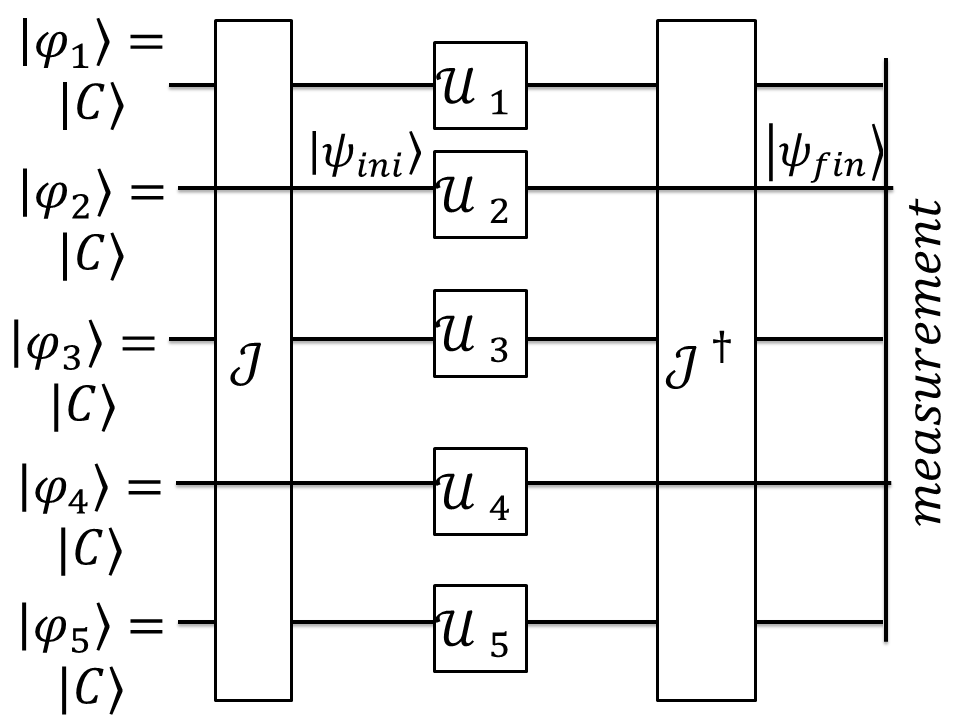
\includegraphics[height=50mm]{Figures/Cover/esquema.png}  \end{center} % gr�ficos
~\\ \vspace{5mm}
\begin{centering}
\LARGE \textbf{Quantum Pirates}
\\ \vspace{5mm}
\Large A Quantum Game-Theory Approach to The Pirate Game
\\ \vspace{15mm}
\Large \textbf{Daniela Filipa Pedro Fontes}
\\ \vspace{15mm}
\large Dissertation for the achievement of the degree
%Disserta\c{c}\~{a}o para obter o grau de Mestre em 
\\ \vspace{2mm}
\LARGE \textbf{Master in Information System and Computer Engineering}
%Engenharia Inform\'{a}tica e de Computadores}
\\ \vspace{20mm}

\Large \textbf{Committee}
%J\'{u}ri}
\\ \vspace{7mm}
\begin{tabular}{lcl}
\large President: 	&   & \large \\ 
\large Advisor:   &Prof. Andreas Wichert& \large \\ 
\large Observer:	 				&   & \large \\
\end{tabular}
 
\vspace{7mm}

%\Large \textbf{\todaythesis\today} \\
\Large \textbf{Outubro 2013} \\
\end{centering}
\let\thepage\relax
\end{flushleft}
\pagebreak


\clearpage
% Since I am using double sided pages, the second page should be white.
% Remember that when delivering the dissertation, IST requires for the cover to appear twice.

\thispagestyle{empty}
\cleardoublepage

\setcounter{page}{1} \pagenumbering{roman}

\baselineskip 18pt % line spacing: -12pt for single spacing
                   %               -18pt for 1 1/2 spacing
                   %               -24pt for double spacingnts} % Uncomment for normal cover with IST logo.
\thispagestyle{empty}
\hbox{} \vfill
\begin{flushright}
%\small \textit{\textbf{Anyone who has never made a mistake has never tried anything new.}}
%\\ \vspace{2mm}  
%\scriptsize Albert Einstein
\small \textit{\textbf{I can live with doubt and uncertainty and not knowing. I think it is much more interesting to live not knowing than to have answers that might be wrong. If we will only allow that, as we progress, we remain unsure, we will leave opportunities for alternatives. We will not become enthusiastic for the fact, the knowledge, the absolute truth of the day, but remain always uncertain... In order to make progress, one must leave the door to the unknown ajar.
}}
\\ \vspace{2mm}  
\scriptsize Richard P. Feynman
\end{flushright}

\clearpage
\thispagestyle{empty}
\cleardoublepage

\pdfbookmark{Acknowledgments}{Acknowledgements}
\begin{acknowledgments} 

 I heard the term ``Quantum Computing'' for the first time at a presentation in the Department of Physics of the University of Coimbra, and the idea of using particles to simulate physical systems and outperform some classical algorithms fascinated me ever since. 

This work is a story of a path started naively our of curiosity for the world around me, a path filled hardships but also ripe with good moments.
This journey was marked by self-doubt, but it was also rich in moments where wonderful travel companions walked alongside giving me strength to carry on. I want to thank all these travel companions.

Namely I would like to thank my advisor, Professor Andreas Wichert, for giving me the freedom to fail and learn from my mistakes, while teaching me how to make Science. 

I would also like to thank my co-workers at Connect Coimbra for teaching me how to balance work and life, and the desire to make a difference in my community.

Last but definitely not the least I give thanks to my loved ones who never ceased supporting me. 
 
\end{acknowledgments}
\clearpage
\thispagestyle{empty}
\cleardoublepage
\begin{abstract}

In this document, we develop a model and a simulation of a quantization scheme for the mathematical puzzle created by Omohundro and Stewart - ``A puzzle for pirates '', also known as Pirate Game. This game is a multi-player version of the game ``Ultimatum '', where the players (Pirates), must distribute fixed number of gold coins acording to some rules.

The Quantum Theory of Games is a field that seeks to introduce the mathematical formalism of Quantum Mechanics in order to explore models of conflict that arise when rational beings make decisions. These models of conflict are pervasive in the structural make-up of our society. The combination of game theory and Quantum Probability, despite not having a practical application, can help in the development of new quantum algorithms. Furthermore the fact that Game Theory is transversal to many areas of knowledge can provide insights to future application of these models.

In this dissertation we focused on the role of quantum entanglement and the use of quantum strategies in the game system. We found that when there is no entanglement the game behaved as the original problem even when the players adopted quantum strategies. When using a unrestricted strategic space and the game system is maximally entangled we found that the game is strictly determined (like the original problem). We also found that when only a the captain has access to quantum strategies in the Pirate Game, she can obtain all the gold coins. These results corroborate similar findings in the field.


\end{abstract}
\begin{keywords}
palavrachave1, palavrachave2, palavrachave3 em ingl\^{e}s
\end{keywords}
\clearpage
\thispagestyle{empty}
\cleardoublepage
\begin{resumo}

Neste trabalho desenvolvemos e simul\'{a}mos um modelo qu\^{a}tico para o puzzle matem\'{a}tico criado por Omohundro e Stewart, ``Um puzzle para piratas''(original em ingl\^{e}s ``A Puzzle for Pirates''). Este jogo consiste numa vers\~{a}o multi-jogador do jogo ``Ultimato''. 

A Teoria de Jogos Qu\^{a}ntica \'{e} uma \'{a}rea que procura introduzir o formalismo matem\'{a}tico na base da Mec\^{a}nica Qu\^{a}ntica para explorar modelos de conflito que surgem quando seres racionais tomam decis\~{o}es. Estes modelos de conflito est\~{a}o na base da estrutura da nossa sociedade. A combina\c{c}\~{a}o de Teoria de Jogos e a Teoria de Probabilidade Qu\^{a}ntica apesar de ainda n\~{a}o ter uma aplica\c{c}\~{a}o pr\'{a}tica pode ajudar no desenvolvimento de novos algoritmos qu\^{a}nticos. O facto da Teoria de Jogos ser ruma disciplina transversal a muitas \'{a}reas do conhecimento pode fazer com que estes modelos possam eventualmente vir a ter relev\^{a}ncia.

Foc\'{a}mo-nos sobretudo no papel do fen\'{o}meno qu\^{a}ntico entrela\c{c}amento no sistema do jogo. Verific\'{a}mos que este fen\'{o}meno introduz varia\c{c}\~{o}es na utilidade esperada pelos jogadores, para algumas estrat\'{e}gias \`{a} semelhan\c{c}a de outros modelos na \'{a}rea. Contudo também verific\'{a}mos a exist\^{e}ncia de estrat\'{e}gias nas quais n\~{a}o existe interfer\^{e}ncia.



\end{resumo}
\begin{palavraschave}
Teoria de Jogos Qu\^antica; Jogo dos Piratas; Mec\^anica Qu\^antica; Teoria de Jogos; Computa\c{c}\~{a}o Qu\^{a}ntica; Teoria de Probabilidade
\end{palavraschave}
\clearpage
\thispagestyle{empty}
\cleardoublepage
% This is required for the fancy chapters
\dominitoc
\dominilof
\dominilot

%%%%%%%%%%%%%%%%%%%%%%%%%%%%%%%%%%%%%%%%%%%%%%%%%%%%%%%%%%%%%%%%%%%%%%
% List of contents
%\renewcommand{\baselinestretch}{1}
\pdfbookmark[0]{Index}{index}
\pdfbookmark[1]{Contents}{toc}
\tableofcontents
% \contentsline{chapter}{References}{\pageref{bib}}
\clearpage
\thispagestyle{empty}
\cleardoublepage
%\renewcommand{\baselinestretch}{1.5}
%%%%%%%%%%%%%%%%%%%%%%%%%%%%%%%%%%%%%%%%%%%%%%%%%%%%%%%%%%%%%%%%%%%%%%
% List of figures
\pdfbookmark[1]{List of Figures}{lof}
\listoffigures
\clearpage
\thispagestyle{empty}
\cleardoublepage

%%%%%%%%%%%%%%%%%%%%%%%%%%%%%%%%%%%%%%%%%%%%%%%%%%%%%%%%%%%%%%%%%%%%%%
% List of tables
\pdfbookmark[1]{List of Tables}{lot}
\listoftables
\clearpage
\thispagestyle{empty}
\cleardoublepage

% %%%%%%%%%%%%%%%%%%%%%%%%%%%%%%%%%%%%%%%%%%%%%%%%%%%%%%%%%%%%%%%%%%%%%%
% % List of algorithms
% Requires packages algorithmic, algorithm
% \pdfbookmark[1]{List of Algorithms}{loa}
% \listofalgorithms
% \cleardoublepage
\acresetall
% %%%%%%%%%%%%%%%%%%%%%%%%%%%%%%%%%%%%%%%%%%%%%%%%%%%%%%%%%%%%%%%%%%%%%%
 % List of acronyms
\pdfbookmark[1]{List of Acronyms}{loac}

\chapter*{Abbreviations}
% See more at http://staff.science.uva.nl/~polko/HOWTO/LATEX/acronym.html
%


\acrodef{CLT}{Central Limit Theorem}
\textbf{\acs{CLT}} - \acl{CLT} \\

%(Examples below:) \\



\clearpage
\thispagestyle{empty}
\cleardoublepage




%%%%%%%%%%%%%%%%%%%%%%%%%%%%%%%%%%%%%%%%%%%%%%%%%%%%%%%%%%%%%%%%%%%%%%
% List of symbols
\pdfbookmark[1]{List of Symbols}{los}



\listofsymbols


%\nomenclature{$A_i$}{Area of the $i^{th}$ component}

%\printnomenclature


%\begin{longtable}[l]{p{50pt} p{100pt}} 
%RAC & Rear axle carrier \\ 
%FAC & Front axle carrier \\
%\end{longtable}

\textbf{Standard Notation}

\renewcommand*{\arraystretch}{1.4}
\begin{longtable}[l]{p{50pt} p{300pt}} 

$\mathbf{i}$
&
 is the imaginary constant $\sqrt{-1}$.
\\
$e$ 
&
is natural constant $2.71828...$
\\
$\vert x \vert $
&
 represents the absolute value of $x$
\\
$\mathbb{R}$ 
&
represents the real numbers.
\\
$\mathbb{C}$ 
&
represents the complex numbers.
\\
$P(A)$ 
& 
represents the probability of an event $A$ occurring.
\\
\end{longtable}
\textbf{Sets and Spaces}

\renewcommand*{\arraystretch}{1.4}
\begin{longtable}[l]{p{50pt} p{300pt}}

$\mathcal{H}^{n}$ 
&
represents a $n$-dimension Hilbert Space.
\\
$\mathcal{B}$ & $= \{ \vert b_{i} \rangle, i=0, n-1\}$

 is a set of orthonormal basis.
\\
\end{longtable}

\textbf{Vectors}

\renewcommand*{\arraystretch}{1.4}
\begin{longtable}[l]{p{50pt} p{300pt}}

$\vert \psi \rangle$
&
 is a quantum state labeled $\psi$ represented by an abstract vector, can also be represented by a $n \times 1$ matrix relative to a basis $\mathcal{B}$.
\\
$\otimes$
&
 represents the tensor product between two vectors.
\\
$ \vert 0 \rangle , \vert 1 \rangle$
&
 are the standard basis for a two-state quantum system (qubit).
\\
\end{longtable}

\textbf{Matrices}

\renewcommand*{\arraystretch}{1.4}
\begin{longtable}[l]{p{50pt} p{300pt}}

$exp(A)$
&
, where A is a square matrix, is a matrix exponential function, equivalent to $e^{A}$.
\\
$\vert A \vert$
&
determinant of the matrix A.
\\
$I$ 
&
represents a $2 \times 2$ identity matrix.
\\
$\sigma_{x}, \sigma_{y}, \sigma_{z}$
&
 are $2 \times 2$ matrices that form a set known as Pauli Operators.
\\
$C, D$
&
 represent Cooperate and Defect strategies in a game, in a quantum game theory environment they are $2 \times 2$ matrices.
\\
$\rho$
&
 represents a density matrix.
\\
$\mathcal{U}$
&
 is a unitary matrix.
\\
$\mathcal{U}^{-1}$
& is the inverse of the unitary matrix $\mathcal{U}$.
\\
$\mathcal{U}^{*}$
&
 is the conjugate of $\mathcal{U}$.
\\
$\mathcal{U}^{T}$
&
 is the transpose of $\mathcal{U}$.
\\
$\mathcal{U}^{\dagger}$
&
 is the conjugate transpose of $\mathcal{U}$.
\\
$\otimes$ &
 represents the Kronecker product between two matrices.
\\
\end{longtable}

\textbf{Game Theory}
\begin{longtable}[l]{p{50pt} p{300pt}}

$\Gamma$ &
 represents a game.
\\
$N$
&
 in a game denotes the number of players.
\\
$u_{i}(A)$ &
 is the expected utility for player $i$ when the outcome $A$ occurs.
\\
$E_{i}$
& is utility functional that specifies the expected utility in a quantum game.
\\
\end{longtable}
\clearpage
\thispagestyle{empty}

\cleardoublepage

%\pagestyle{document}%Fancy head and foot with lines
\pagestyle{documentsimple}%Simple head
% %%%%%%%%%%%%%%%%%%%%%%%%%%%%%%%%%%%%%%%%%%%%%%%%%%%%%%%%%%%%%%%%%%%%%%
% Dummy Chapter:
% %%%%%%%%%%%%%%%%%%%%%%%%%%%%%%%%%%%%%%%%%%%%%%%%%%%%%%%%%%%%%%%%%%%%%%

% %%%%%%%%%%%%%%%%%%%%%%%%%%%%%%%%%%%%%%%%%%%%%%%%%%%%%%%%%%%%%%%%%%%%%%
% The Introduction:
% %%%%%%%%%%%%%%%%%%%%%%%%%%%%%%%%%%%%%%%%%%%%%%%%%%%%%%%%%%%%%%%%%%%%%%
\fancychapter{Quantum Pirate Game}
\label{cap:chapter4}

\textit{In this chapter we describe the Pirate Game and the steps to model a quantum approach to the problem. }




\section{Pirate Game}
\label{sec:pirate}

\begin{emph}
On selecting the problem...
\end{emph}


\subsection{Problem Description}
\label{subsec:description}

The original Pirate Game is a multiplayer version of the Ultimatum game that is usually stated as follows:

\begin{quotation}
Suppose there are 5 rational pirates: A; B; C; D; E. The pirates have a  loot of 100 indivisible gold coins to divide among themselves.


As the pirates have a strict hierarchy, in which pirate A is the captain and E has the lowest rank, the highest ranking pirate alive will propose a division. Then each pirate will cast a vote on whether or not to accept the proposal. 

If a majority or a tie is reached the goods will be allocated according to the proposal. Otherwise the proposer will be thrown overboard and the next pirate in the hierarchy assumes the place of the captain. 

We consider that each pirate privileges her survival, and then will want to maximize the number of coins received. When the result is indifferent the pirates prefer to throw another pirate overboard and thus climbing in the hierarchy. 
\end{quotation}

We can arrive at an equilibrium in this problem by using backward induction. At the end of the problem, supposing there are two pirates left, the decisions are very straight forward. As the highest ranking pirate can pass the proposal without the remaining friend, her self-interest dictates that she will get the 100 gold coins. Knowing this, pirate E knows that any bribe other higher ranking pirate offers her will leave her better than if the game arrives to the last proposal. 

\begin{table}
\begin{center}
\begin{tabular}{cc}
  \num\putindeepbox[7pt]{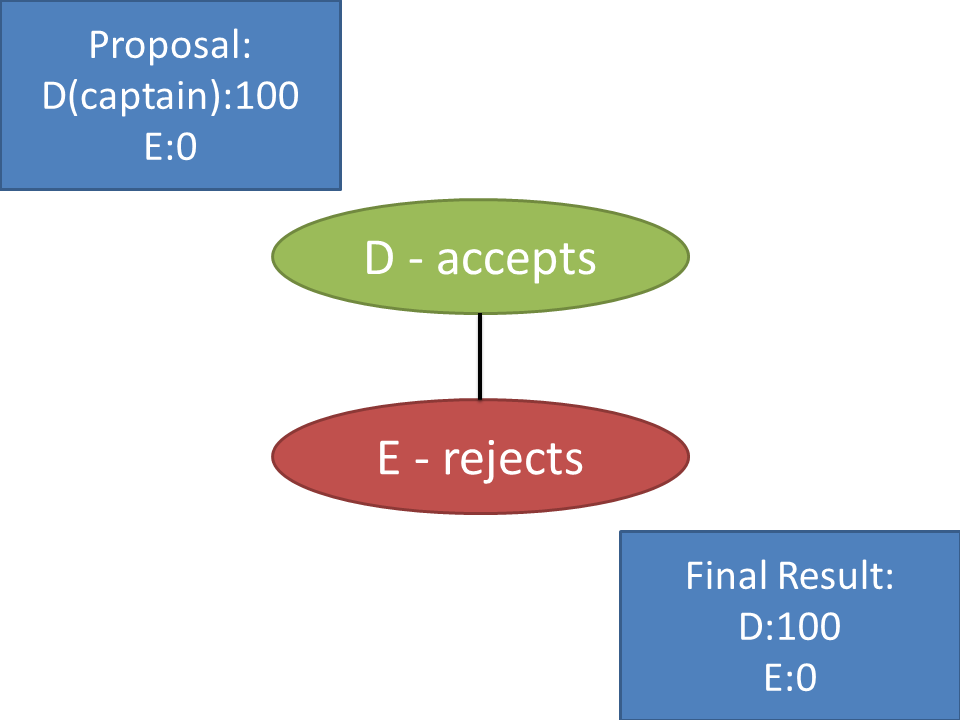
\includegraphics[scale=0.20]{Pirates1/Slide1.PNG}}
    & \num\putindeepbox[7pt]{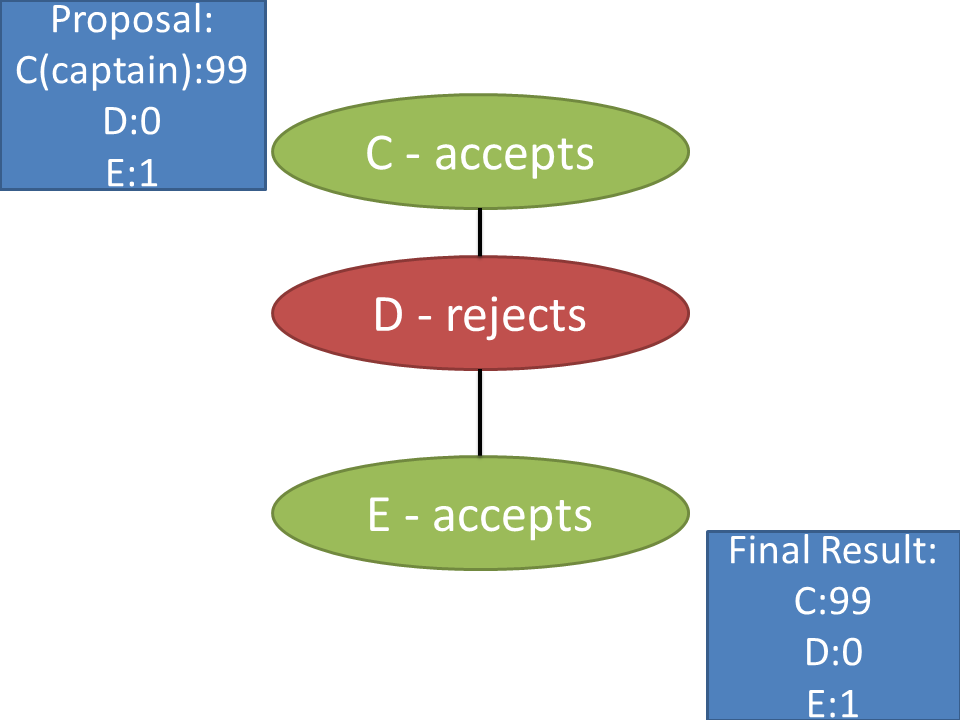
\includegraphics[scale=0.20]{Pirates1/Slide2.PNG}} \\
  \num\putindeepbox[7pt]{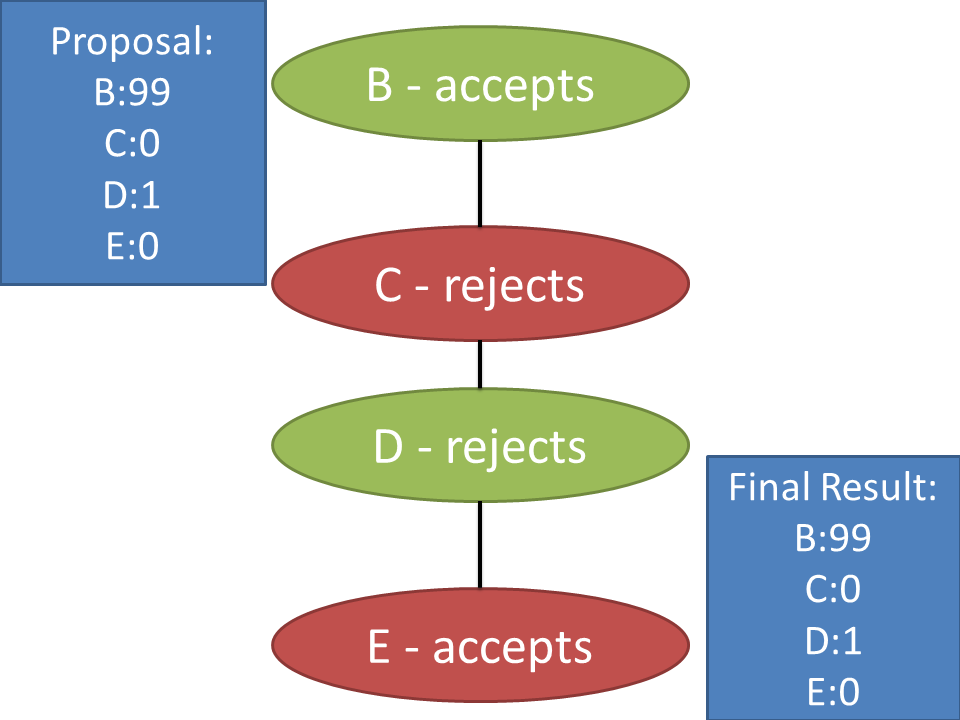
\includegraphics[scale=0.20]{Pirates1/Slide3.PNG}}
    & \num\putindeepbox[7pt]{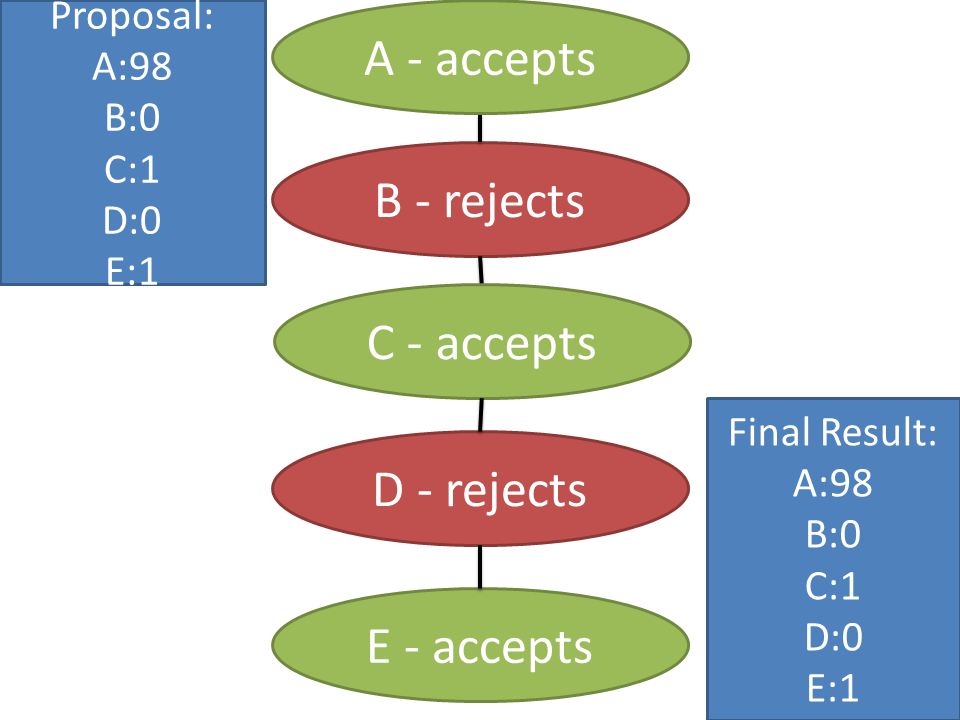
\includegraphics[scale=0.20]{Pirates1/Slide4.PNG}} \\
\end{tabular}
\caption{The equilibrium for the Pitrate Game can be found through backward induction. From a), where there's only two pirates left, to d), that corresponds to the initial problem we define the best response.}
\label{tab:piratas_m}
\end{center}
 \end{table}

When applying this reasoning to the three pirate move, as pirate C knows she needs one more vote to pass her proposal and avoiding death, she will offer the minimum amount of coins that will make pirate E better off than if it comes to the last stage with two pirates. This means that pirate C will offer 1 gold coin to pirate E, and keep the remaining 99 coins. 

With 4 pirates, B would rather bribe pirate D with 1 gold coin, because E would rather like climb on the hierarchy and getting the same payoff. Finaly, with 5 pirates the captain (A), will keep 98 gold coins and rely on pirate C and E to vote in favor of the proposal, by giving 1 gold coin each.

We can generalize this problem for $N$ pirate. If we assign a number to each pirate, where the captain is number 1 and the lower the number the higher the rank. If the number of coins is superior to the number of pirates, the equilibrium will have the captain (highest ranking pirate), giving a gold coin to each odd pirate, in case the number of players alive is odd, while keeping the rest to herself. When we have a even number of players the captain will assign a gold peice to each pirate with a even number, and the the remaining coins to herself.




\subsection{Quantum considerations}
\label{subsec:description_2}

In order to model the mencioned problem it's helpful to define it using the definition of quantun game ($\Gamma$), referred in \ref{eq:quantum_game_six_tuple}, Section \ref{sec:background_quantum_game_theory}.
In terms of mechanics and steps, this problem could be described using 3 players and later extended to any number $N$ of players. 

We begin by assigning an offset to each pirate in order to identify it, as in the Section \label{subsec:description}. So the captain is number 1 and the lower the number the higher the rank. 

Each player will be able to manipulate a qubit in the system, in this case $\vert\varphi_{1}\rangle,\:\vert\varphi_{2}\rangle,$ and $\vert\varphi_{3}\rangle$, with one of two operators \ref{eq:operators_piratas_quanticos}. The two operators will correspond to the action of voting ``Yes'' or to Cooperate, and voting ``No'', meaning that they won't accept the proposal. For the defection operator ($D$), we chose one of Pauli's Operators - the Bit-flip operator. The cooperation operator will be represented by the Identity operator. 

\begin{equation}
\label{eq:operators_piratas_quanticos}
\mathcal{U}_{i} = \begin{cases}
C = o_{i0}=\left[\begin{array}{cc}
1 & 0\\
0 & 1
\end{array}\right]\\
D = o_{i1}=\left[\begin{array}{cc}
0 & 1\\
1 & 0
\end{array}\right]
\end{cases} , i \in \{ 1, 2, 3 \}
\end{equation}

 The highest ranking pirate in the hierachy will be responsible to make a proposal. This proposal can be modelled as describing the payoff functionals for every pirate, according to some rules. This goods allocation proposal will be executed if there is a majority (or a tie), in the voting step. In the voting step, each pirate will cast a vote by choosing simultaneously a operator (that can mean either accept or reject the proposal).

''''''Depending on the measurement outcome that occurs with probability x, the players will act on the second round. The Luders rule is applied here. The highest ranking player will no longer have access to the voting operators, instead he will only be able to manipulate de system using a symetric matrix like a coin operator, in order to not affect the voting.

Keeping the system in a higher dimension is considered because of the following reasons: We don't have proof that the states are separable. There are various mappings that fit the system composition. 


Initial state: variable to study.
Payoff functions: variable to study.

\begin{emph}
One important aspect is that the payoff functional changes
\end{emph}
%\section{Section B}
\label{sec:sectionb}

\subsection{Subsection A}
\label{subsec:subasectionB}

The model described can also be represented as

\begin{equation}
\dot{\mathbf{x}}(t) = \mathbf{T}\mathbf{z}(y),\  \mathbf{y}(0) = \mathbf{y}_0,\  z\geq 0 \\
\label{eq:dummyeq1}
\end{equation}

\noindent where

\begin{equation}
\mathbf{A} = \left[ \begin{array}{cc} -(a_{12} + a_{10}) & a_{21} \\ a_{12} & -(a_{21} + a_{20}) \end{array} \right],\ \mathbf{x} = \left[ \begin{array}{c} x_1 \\ x_2 \end{array} \right] \\
\label{eq:dummyeq2}
\end{equation}


\subsection{Subsection B}
\label{subsec:subbsectionB}

\begin{table}[H]
	\centering
	\caption{Dummy Table.}
	\begin{tabular}{|c|c|c|c|} \hline
		\textbf{Vendor Name} 				& \textbf{Short Name}	& \textbf{Commercial Name}	& \textbf{Manufacturer}	\\ \hline \hline
		\multirow{3}{*}{Text in Multiple Row}		&	ABC				&  ABC\textreg				& ABC SA			         \\ \cline{2-4}
		 								&        DEF				&  DEF\textreg				& DEF SA				\\ \cline{2-4}
										&        GHF			&  GHF\textreg				& GHF SA				\\ \hline
		Text in Single Row					&        IJK				& IJK\textreg				& IJK SA				\\ \hline
		Frescos SA						&        LMN			& LMN\textreg				& LMN SA				\\ \hline
		Carros Lda.						&    \multicolumn{3}{|c|}{Text in Multiple Column}							\\ \hline
	\end{tabular}
	\label{tab:dummytable}
\end{table}
\cleardoublepage
% %%%%%%%%%%%%%%%%%%%%%%%%%%%%%%%%%%%%%%%%%%%%%%%%%%%%%%%%%%%%%%%%%%%%%%
% Dummy Chapter:
% %%%%%%%%%%%%%%%%%%%%%%%%%%%%%%%%%%%%%%%%%%%%%%%%%%%%%%%%%%%%%%%%%%%%%%

% %%%%%%%%%%%%%%%%%%%%%%%%%%%%%%%%%%%%%%%%%%%%%%%%%%%%%%%%%%%%%%%%%%%%%%
% The Introduction:
% %%%%%%%%%%%%%%%%%%%%%%%%%%%%%%%%%%%%%%%%%%%%%%%%%%%%%%%%%%%%%%%%%%%%%%
\fancychapter{Quantum Pirate Game}
\label{cap:chapter4}

\textit{In this chapter we describe the Pirate Game and the steps to model a quantum approach to the problem. }




\section{Pirate Game}
\label{sec:pirate}

\begin{emph}
On selecting the problem...
\end{emph}


\subsection{Problem Description}
\label{subsec:description}

The original Pirate Game is a multiplayer version of the Ultimatum game that is usually stated as follows:

\begin{quotation}
Suppose there are 5 rational pirates: A; B; C; D; E. The pirates have a  loot of 100 indivisible gold coins to divide among themselves.


As the pirates have a strict hierarchy, in which pirate A is the captain and E has the lowest rank, the highest ranking pirate alive will propose a division. Then each pirate will cast a vote on whether or not to accept the proposal. 

If a majority or a tie is reached the goods will be allocated according to the proposal. Otherwise the proposer will be thrown overboard and the next pirate in the hierarchy assumes the place of the captain. 

We consider that each pirate privileges her survival, and then will want to maximize the number of coins received. When the result is indifferent the pirates prefer to throw another pirate overboard and thus climbing in the hierarchy. 
\end{quotation}

We can arrive at an equilibrium in this problem by using backward induction. At the end of the problem, supposing there are two pirates left, the decisions are very straight forward. As the highest ranking pirate can pass the proposal without the remaining friend, her self-interest dictates that she will get the 100 gold coins. Knowing this, pirate E knows that any bribe other higher ranking pirate offers her will leave her better than if the game arrives to the last proposal. 

\begin{table}
\begin{center}
\begin{tabular}{cc}
  \num\putindeepbox[7pt]{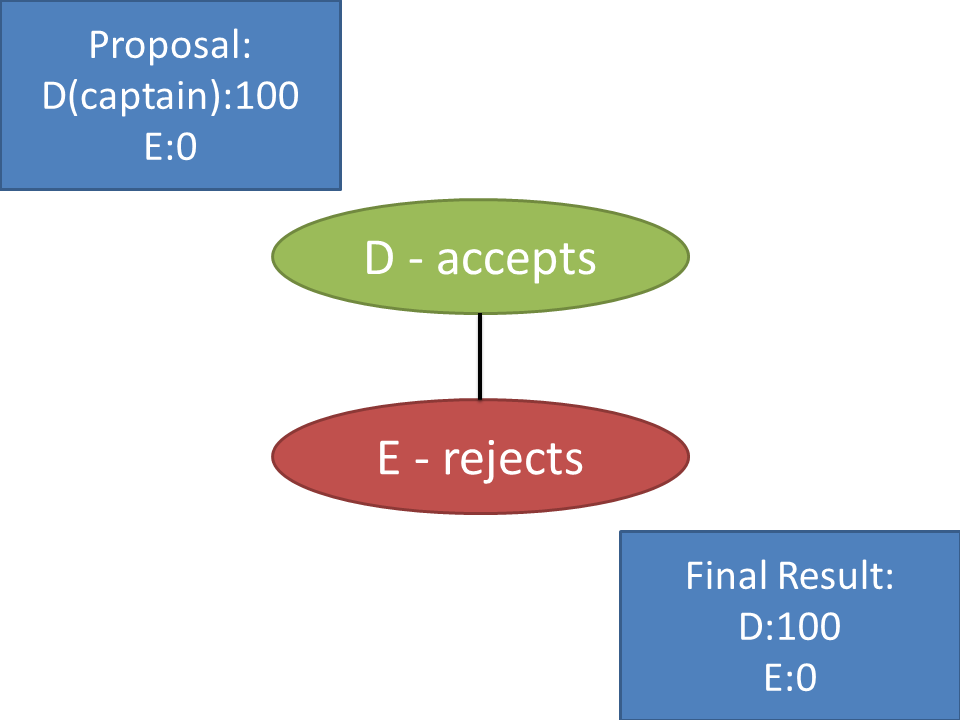
\includegraphics[scale=0.20]{Pirates1/Slide1.PNG}}
    & \num\putindeepbox[7pt]{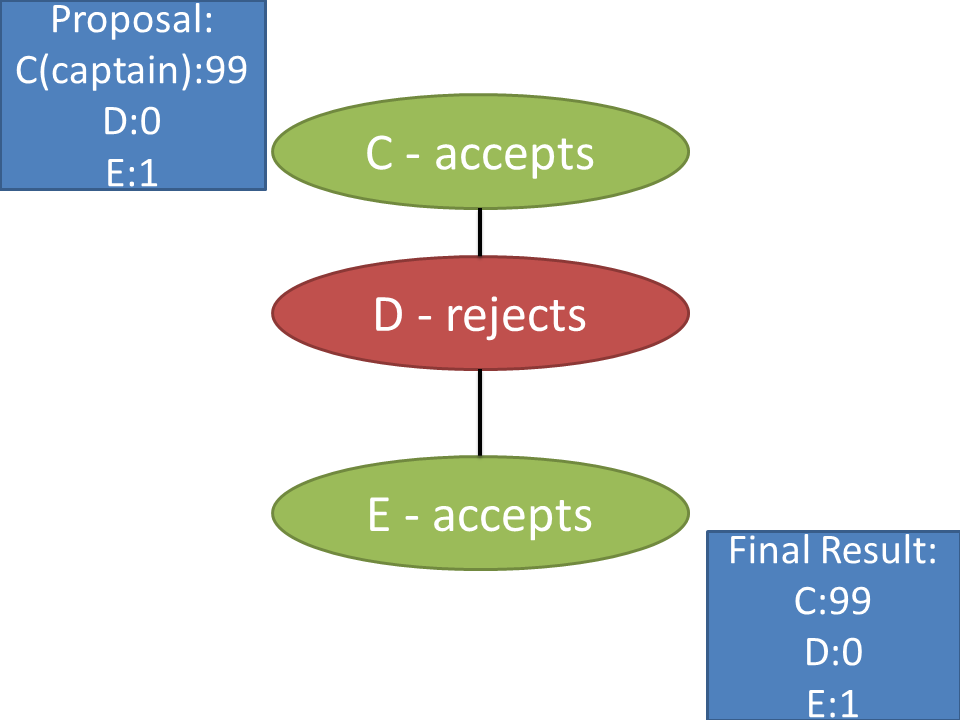
\includegraphics[scale=0.20]{Pirates1/Slide2.PNG}} \\
  \num\putindeepbox[7pt]{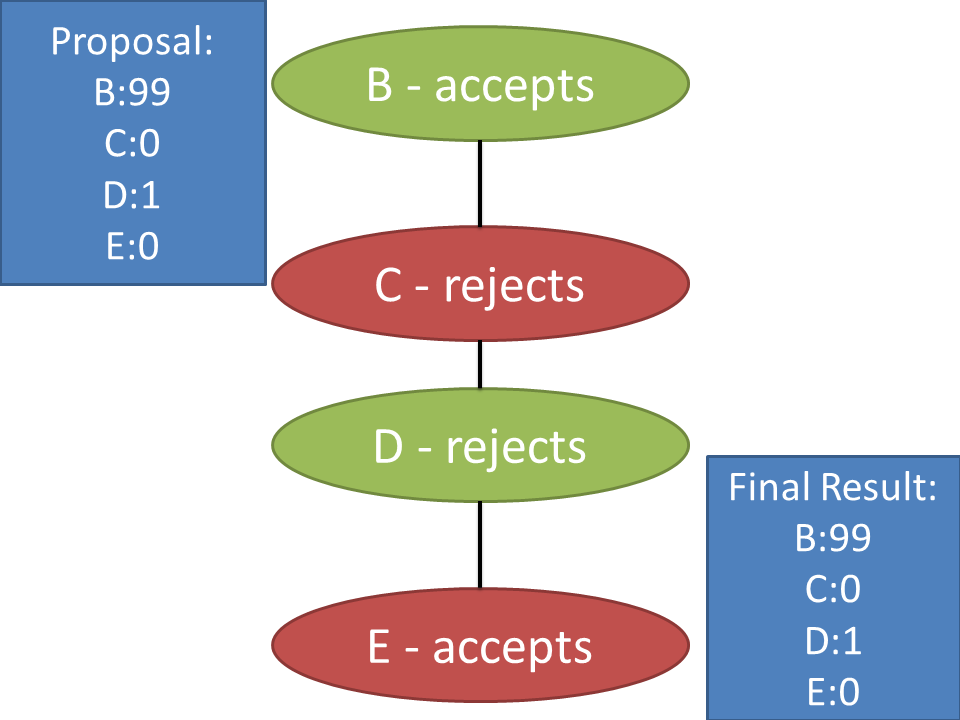
\includegraphics[scale=0.20]{Pirates1/Slide3.PNG}}
    & \num\putindeepbox[7pt]{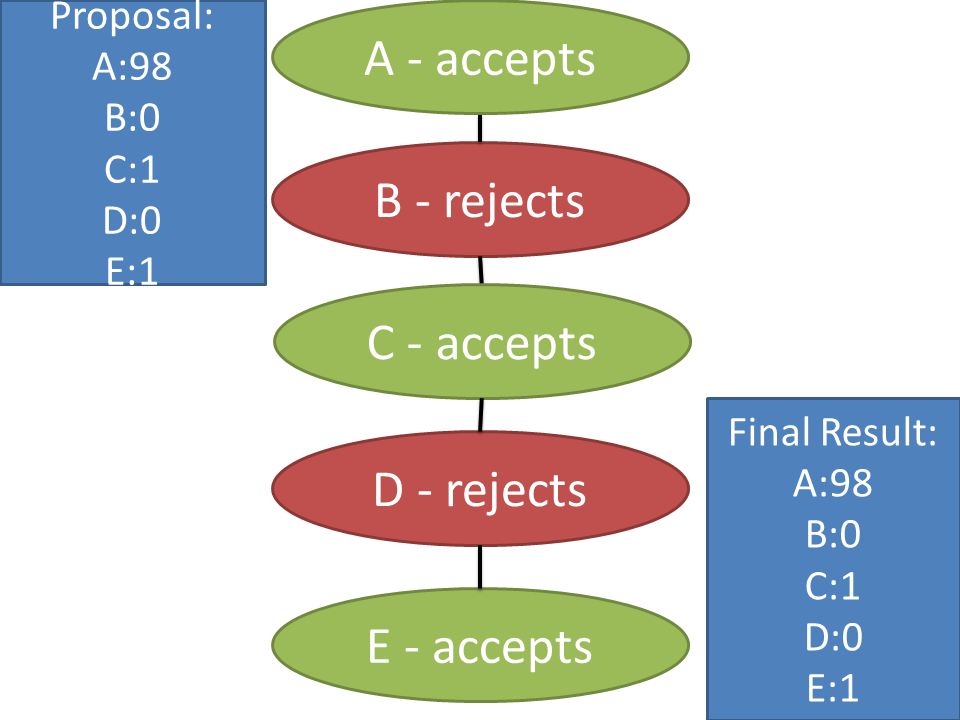
\includegraphics[scale=0.20]{Pirates1/Slide4.PNG}} \\
\end{tabular}
\caption{The equilibrium for the Pitrate Game can be found through backward induction. From a), where there's only two pirates left, to d), that corresponds to the initial problem we define the best response.}
\label{tab:piratas_m}
\end{center}
 \end{table}

When applying this reasoning to the three pirate move, as pirate C knows she needs one more vote to pass her proposal and avoiding death, she will offer the minimum amount of coins that will make pirate E better off than if it comes to the last stage with two pirates. This means that pirate C will offer 1 gold coin to pirate E, and keep the remaining 99 coins. 

With 4 pirates, B would rather bribe pirate D with 1 gold coin, because E would rather like climb on the hierarchy and getting the same payoff. Finaly, with 5 pirates the captain (A), will keep 98 gold coins and rely on pirate C and E to vote in favor of the proposal, by giving 1 gold coin each.

We can generalize this problem for $N$ pirate. If we assign a number to each pirate, where the captain is number 1 and the lower the number the higher the rank. If the number of coins is superior to the number of pirates, the equilibrium will have the captain (highest ranking pirate), giving a gold coin to each odd pirate, in case the number of players alive is odd, while keeping the rest to herself. When we have a even number of players the captain will assign a gold peice to each pirate with a even number, and the the remaining coins to herself.




\subsection{Quantum considerations}
\label{subsec:description_2}

In order to model the mencioned problem it's helpful to define it using the definition of quantun game ($\Gamma$), referred in \ref{eq:quantum_game_six_tuple}, Section \ref{sec:background_quantum_game_theory}.
In terms of mechanics and steps, this problem could be described using 3 players and later extended to any number $N$ of players. 

We begin by assigning an offset to each pirate in order to identify it, as in the Section \label{subsec:description}. So the captain is number 1 and the lower the number the higher the rank. 

Each player will be able to manipulate a qubit in the system, in this case $\vert\varphi_{1}\rangle,\:\vert\varphi_{2}\rangle,$ and $\vert\varphi_{3}\rangle$, with one of two operators \ref{eq:operators_piratas_quanticos}. The two operators will correspond to the action of voting ``Yes'' or to Cooperate, and voting ``No'', meaning that they won't accept the proposal. For the defection operator ($D$), we chose one of Pauli's Operators - the Bit-flip operator. The cooperation operator will be represented by the Identity operator. 

\begin{equation}
\label{eq:operators_piratas_quanticos}
\mathcal{U}_{i} = \begin{cases}
C = o_{i0}=\left[\begin{array}{cc}
1 & 0\\
0 & 1
\end{array}\right]\\
D = o_{i1}=\left[\begin{array}{cc}
0 & 1\\
1 & 0
\end{array}\right]
\end{cases} , i \in \{ 1, 2, 3 \}
\end{equation}

 The highest ranking pirate in the hierachy will be responsible to make a proposal. This proposal can be modelled as describing the payoff functionals for every pirate, according to some rules. This goods allocation proposal will be executed if there is a majority (or a tie), in the voting step. In the voting step, each pirate will cast a vote by choosing simultaneously a operator (that can mean either accept or reject the proposal).

''''''Depending on the measurement outcome that occurs with probability x, the players will act on the second round. The Luders rule is applied here. The highest ranking player will no longer have access to the voting operators, instead he will only be able to manipulate de system using a symetric matrix like a coin operator, in order to not affect the voting.

Keeping the system in a higher dimension is considered because of the following reasons: We don't have proof that the states are separable. There are various mappings that fit the system composition. 


Initial state: variable to study.
Payoff functions: variable to study.

\begin{emph}
One important aspect is that the payoff functional changes
\end{emph}
%\section{Section B}
\label{sec:sectionb}

\subsection{Subsection A}
\label{subsec:subasectionB}

The model described can also be represented as

\begin{equation}
\dot{\mathbf{x}}(t) = \mathbf{T}\mathbf{z}(y),\  \mathbf{y}(0) = \mathbf{y}_0,\  z\geq 0 \\
\label{eq:dummyeq1}
\end{equation}

\noindent where

\begin{equation}
\mathbf{A} = \left[ \begin{array}{cc} -(a_{12} + a_{10}) & a_{21} \\ a_{12} & -(a_{21} + a_{20}) \end{array} \right],\ \mathbf{x} = \left[ \begin{array}{c} x_1 \\ x_2 \end{array} \right] \\
\label{eq:dummyeq2}
\end{equation}


\subsection{Subsection B}
\label{subsec:subbsectionB}

\begin{table}[H]
	\centering
	\caption{Dummy Table.}
	\begin{tabular}{|c|c|c|c|} \hline
		\textbf{Vendor Name} 				& \textbf{Short Name}	& \textbf{Commercial Name}	& \textbf{Manufacturer}	\\ \hline \hline
		\multirow{3}{*}{Text in Multiple Row}		&	ABC				&  ABC\textreg				& ABC SA			         \\ \cline{2-4}
		 								&        DEF				&  DEF\textreg				& DEF SA				\\ \cline{2-4}
										&        GHF			&  GHF\textreg				& GHF SA				\\ \hline
		Text in Single Row					&        IJK				& IJK\textreg				& IJK SA				\\ \hline
		Frescos SA						&        LMN			& LMN\textreg				& LMN SA				\\ \hline
		Carros Lda.						&    \multicolumn{3}{|c|}{Text in Multiple Column}							\\ \hline
	\end{tabular}
	\label{tab:dummytable}
\end{table}
\cleardoublepage
% %%%%%%%%%%%%%%%%%%%%%%%%%%%%%%%%%%%%%%%%%%%%%%%%%%%%%%%%%%%%%%%%%%%%%%
% Dummy Chapter:
% %%%%%%%%%%%%%%%%%%%%%%%%%%%%%%%%%%%%%%%%%%%%%%%%%%%%%%%%%%%%%%%%%%%%%%

% %%%%%%%%%%%%%%%%%%%%%%%%%%%%%%%%%%%%%%%%%%%%%%%%%%%%%%%%%%%%%%%%%%%%%%
% The Introduction:
% %%%%%%%%%%%%%%%%%%%%%%%%%%%%%%%%%%%%%%%%%%%%%%%%%%%%%%%%%%%%%%%%%%%%%%
\fancychapter{Quantum Pirate Game}
\label{cap:chapter4}

\textit{In this chapter we describe the Pirate Game and the steps to model a quantum approach to the problem. }




\section{Pirate Game}
\label{sec:pirate}

\begin{emph}
On selecting the problem...
\end{emph}


\subsection{Problem Description}
\label{subsec:description}

The original Pirate Game is a multiplayer version of the Ultimatum game that is usually stated as follows:

\begin{quotation}
Suppose there are 5 rational pirates: A; B; C; D; E. The pirates have a  loot of 100 indivisible gold coins to divide among themselves.


As the pirates have a strict hierarchy, in which pirate A is the captain and E has the lowest rank, the highest ranking pirate alive will propose a division. Then each pirate will cast a vote on whether or not to accept the proposal. 

If a majority or a tie is reached the goods will be allocated according to the proposal. Otherwise the proposer will be thrown overboard and the next pirate in the hierarchy assumes the place of the captain. 

We consider that each pirate privileges her survival, and then will want to maximize the number of coins received. When the result is indifferent the pirates prefer to throw another pirate overboard and thus climbing in the hierarchy. 
\end{quotation}

We can arrive at an equilibrium in this problem by using backward induction. At the end of the problem, supposing there are two pirates left, the decisions are very straight forward. As the highest ranking pirate can pass the proposal without the remaining friend, her self-interest dictates that she will get the 100 gold coins. Knowing this, pirate E knows that any bribe other higher ranking pirate offers her will leave her better than if the game arrives to the last proposal. 

\begin{table}
\begin{center}
\begin{tabular}{cc}
  \num\putindeepbox[7pt]{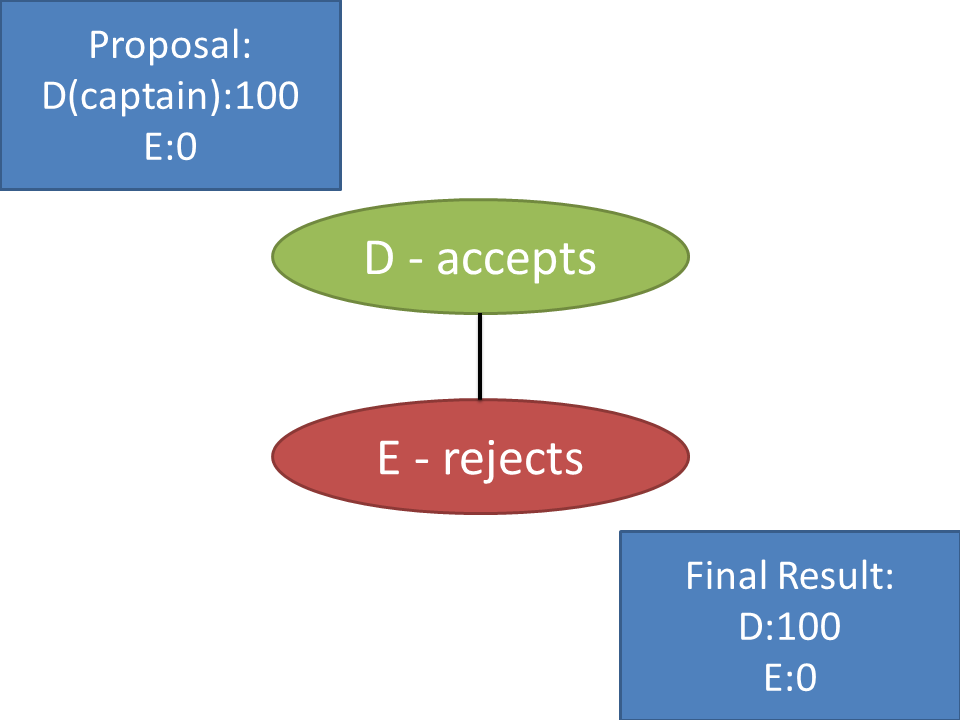
\includegraphics[scale=0.20]{Pirates1/Slide1.PNG}}
    & \num\putindeepbox[7pt]{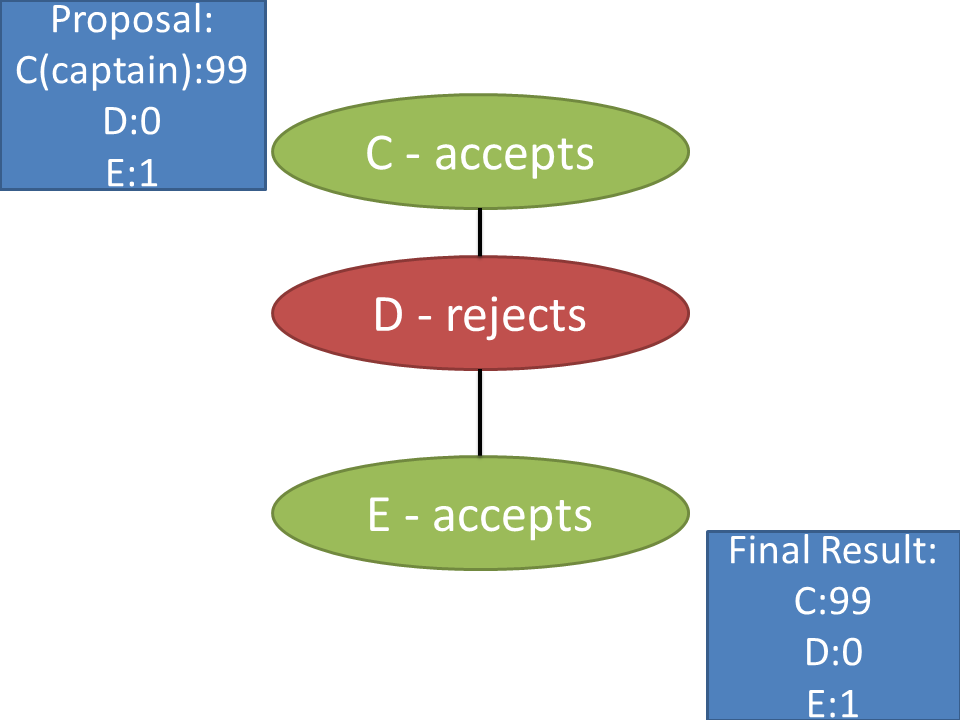
\includegraphics[scale=0.20]{Pirates1/Slide2.PNG}} \\
  \num\putindeepbox[7pt]{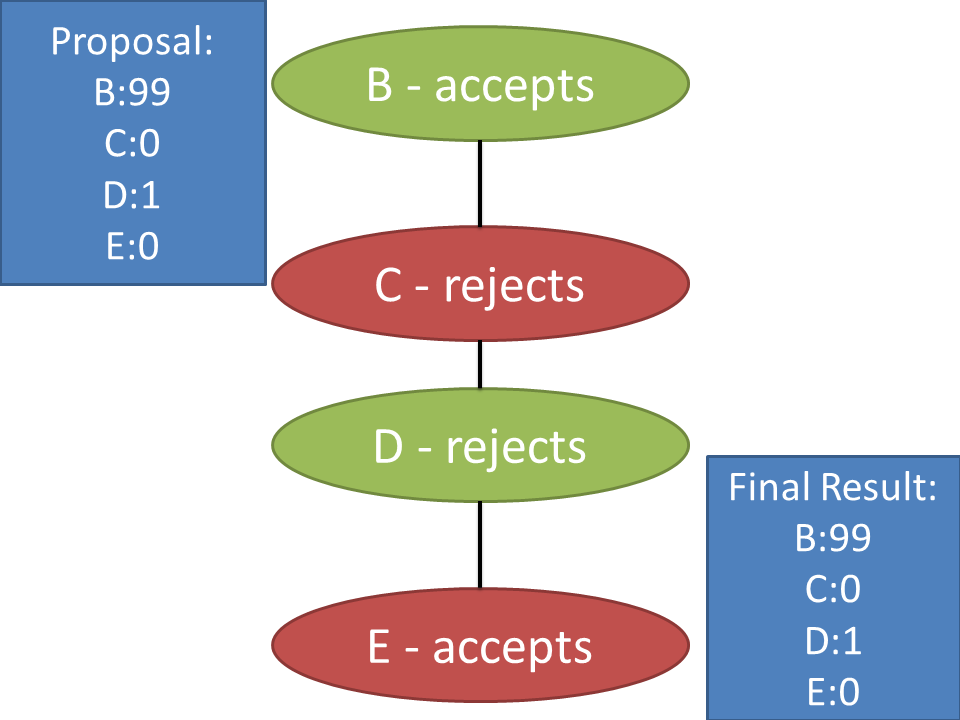
\includegraphics[scale=0.20]{Pirates1/Slide3.PNG}}
    & \num\putindeepbox[7pt]{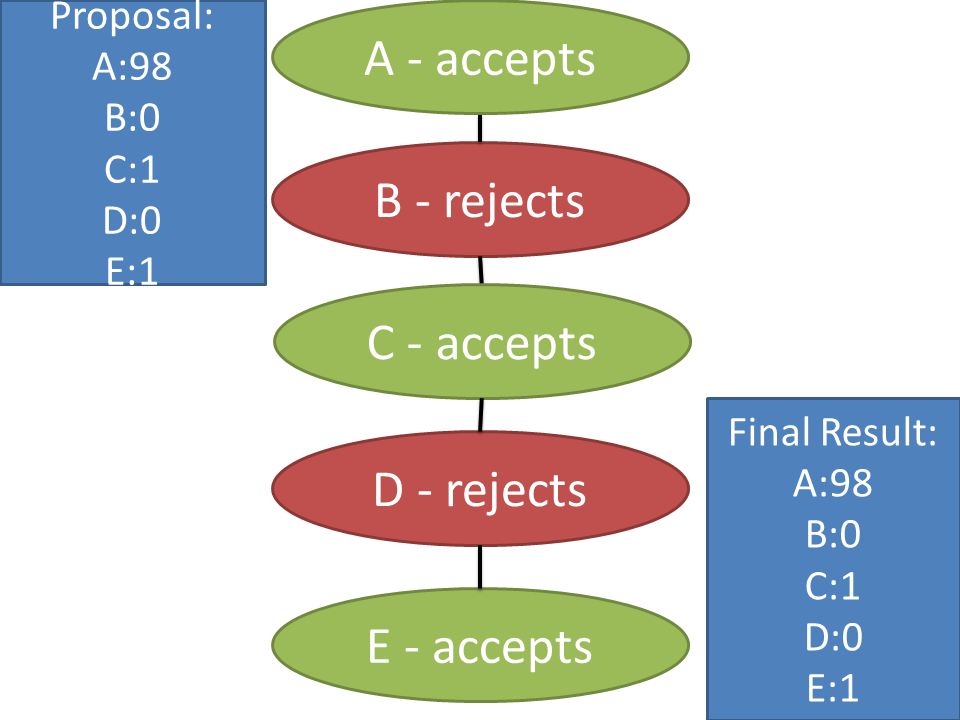
\includegraphics[scale=0.20]{Pirates1/Slide4.PNG}} \\
\end{tabular}
\caption{The equilibrium for the Pitrate Game can be found through backward induction. From a), where there's only two pirates left, to d), that corresponds to the initial problem we define the best response.}
\label{tab:piratas_m}
\end{center}
 \end{table}

When applying this reasoning to the three pirate move, as pirate C knows she needs one more vote to pass her proposal and avoiding death, she will offer the minimum amount of coins that will make pirate E better off than if it comes to the last stage with two pirates. This means that pirate C will offer 1 gold coin to pirate E, and keep the remaining 99 coins. 

With 4 pirates, B would rather bribe pirate D with 1 gold coin, because E would rather like climb on the hierarchy and getting the same payoff. Finaly, with 5 pirates the captain (A), will keep 98 gold coins and rely on pirate C and E to vote in favor of the proposal, by giving 1 gold coin each.

We can generalize this problem for $N$ pirate. If we assign a number to each pirate, where the captain is number 1 and the lower the number the higher the rank. If the number of coins is superior to the number of pirates, the equilibrium will have the captain (highest ranking pirate), giving a gold coin to each odd pirate, in case the number of players alive is odd, while keeping the rest to herself. When we have a even number of players the captain will assign a gold peice to each pirate with a even number, and the the remaining coins to herself.




\subsection{Quantum considerations}
\label{subsec:description_2}

In order to model the mencioned problem it's helpful to define it using the definition of quantun game ($\Gamma$), referred in \ref{eq:quantum_game_six_tuple}, Section \ref{sec:background_quantum_game_theory}.
In terms of mechanics and steps, this problem could be described using 3 players and later extended to any number $N$ of players. 

We begin by assigning an offset to each pirate in order to identify it, as in the Section \label{subsec:description}. So the captain is number 1 and the lower the number the higher the rank. 

Each player will be able to manipulate a qubit in the system, in this case $\vert\varphi_{1}\rangle,\:\vert\varphi_{2}\rangle,$ and $\vert\varphi_{3}\rangle$, with one of two operators \ref{eq:operators_piratas_quanticos}. The two operators will correspond to the action of voting ``Yes'' or to Cooperate, and voting ``No'', meaning that they won't accept the proposal. For the defection operator ($D$), we chose one of Pauli's Operators - the Bit-flip operator. The cooperation operator will be represented by the Identity operator. 

\begin{equation}
\label{eq:operators_piratas_quanticos}
\mathcal{U}_{i} = \begin{cases}
C = o_{i0}=\left[\begin{array}{cc}
1 & 0\\
0 & 1
\end{array}\right]\\
D = o_{i1}=\left[\begin{array}{cc}
0 & 1\\
1 & 0
\end{array}\right]
\end{cases} , i \in \{ 1, 2, 3 \}
\end{equation}

 The highest ranking pirate in the hierachy will be responsible to make a proposal. This proposal can be modelled as describing the payoff functionals for every pirate, according to some rules. This goods allocation proposal will be executed if there is a majority (or a tie), in the voting step. In the voting step, each pirate will cast a vote by choosing simultaneously a operator (that can mean either accept or reject the proposal).

''''''Depending on the measurement outcome that occurs with probability x, the players will act on the second round. The Luders rule is applied here. The highest ranking player will no longer have access to the voting operators, instead he will only be able to manipulate de system using a symetric matrix like a coin operator, in order to not affect the voting.

Keeping the system in a higher dimension is considered because of the following reasons: We don't have proof that the states are separable. There are various mappings that fit the system composition. 


Initial state: variable to study.
Payoff functions: variable to study.

\begin{emph}
One important aspect is that the payoff functional changes
\end{emph}
%\section{Section B}
\label{sec:sectionb}

\subsection{Subsection A}
\label{subsec:subasectionB}

The model described can also be represented as

\begin{equation}
\dot{\mathbf{x}}(t) = \mathbf{T}\mathbf{z}(y),\  \mathbf{y}(0) = \mathbf{y}_0,\  z\geq 0 \\
\label{eq:dummyeq1}
\end{equation}

\noindent where

\begin{equation}
\mathbf{A} = \left[ \begin{array}{cc} -(a_{12} + a_{10}) & a_{21} \\ a_{12} & -(a_{21} + a_{20}) \end{array} \right],\ \mathbf{x} = \left[ \begin{array}{c} x_1 \\ x_2 \end{array} \right] \\
\label{eq:dummyeq2}
\end{equation}


\subsection{Subsection B}
\label{subsec:subbsectionB}

\begin{table}[H]
	\centering
	\caption{Dummy Table.}
	\begin{tabular}{|c|c|c|c|} \hline
		\textbf{Vendor Name} 				& \textbf{Short Name}	& \textbf{Commercial Name}	& \textbf{Manufacturer}	\\ \hline \hline
		\multirow{3}{*}{Text in Multiple Row}		&	ABC				&  ABC\textreg				& ABC SA			         \\ \cline{2-4}
		 								&        DEF				&  DEF\textreg				& DEF SA				\\ \cline{2-4}
										&        GHF			&  GHF\textreg				& GHF SA				\\ \hline
		Text in Single Row					&        IJK				& IJK\textreg				& IJK SA				\\ \hline
		Frescos SA						&        LMN			& LMN\textreg				& LMN SA				\\ \hline
		Carros Lda.						&    \multicolumn{3}{|c|}{Text in Multiple Column}							\\ \hline
	\end{tabular}
	\label{tab:dummytable}
\end{table}
\cleardoublepage
% %%%%%%%%%%%%%%%%%%%%%%%%%%%%%%%%%%%%%%%%%%%%%%%%%%%%%%%%%%%%%%%%%%%%%%
% Dummy Chapter:
% %%%%%%%%%%%%%%%%%%%%%%%%%%%%%%%%%%%%%%%%%%%%%%%%%%%%%%%%%%%%%%%%%%%%%%

% %%%%%%%%%%%%%%%%%%%%%%%%%%%%%%%%%%%%%%%%%%%%%%%%%%%%%%%%%%%%%%%%%%%%%%
% The Introduction:
% %%%%%%%%%%%%%%%%%%%%%%%%%%%%%%%%%%%%%%%%%%%%%%%%%%%%%%%%%%%%%%%%%%%%%%
\fancychapter{Quantum Pirate Game}
\label{cap:chapter4}

\textit{In this chapter we describe the Pirate Game and the steps to model a quantum approach to the problem. }




\section{Pirate Game}
\label{sec:pirate}

\begin{emph}
On selecting the problem...
\end{emph}


\subsection{Problem Description}
\label{subsec:description}

The original Pirate Game is a multiplayer version of the Ultimatum game that is usually stated as follows:

\begin{quotation}
Suppose there are 5 rational pirates: A; B; C; D; E. The pirates have a  loot of 100 indivisible gold coins to divide among themselves.


As the pirates have a strict hierarchy, in which pirate A is the captain and E has the lowest rank, the highest ranking pirate alive will propose a division. Then each pirate will cast a vote on whether or not to accept the proposal. 

If a majority or a tie is reached the goods will be allocated according to the proposal. Otherwise the proposer will be thrown overboard and the next pirate in the hierarchy assumes the place of the captain. 

We consider that each pirate privileges her survival, and then will want to maximize the number of coins received. When the result is indifferent the pirates prefer to throw another pirate overboard and thus climbing in the hierarchy. 
\end{quotation}

We can arrive at an equilibrium in this problem by using backward induction. At the end of the problem, supposing there are two pirates left, the decisions are very straight forward. As the highest ranking pirate can pass the proposal without the remaining friend, her self-interest dictates that she will get the 100 gold coins. Knowing this, pirate E knows that any bribe other higher ranking pirate offers her will leave her better than if the game arrives to the last proposal. 

\begin{table}
\begin{center}
\begin{tabular}{cc}
  \num\putindeepbox[7pt]{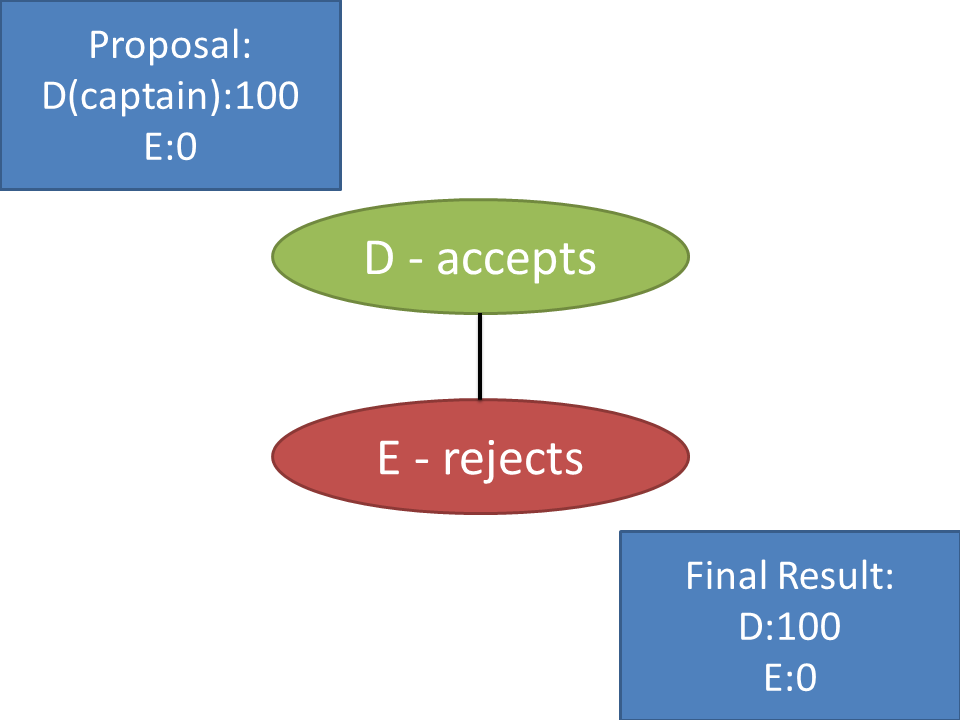
\includegraphics[scale=0.20]{Pirates1/Slide1.PNG}}
    & \num\putindeepbox[7pt]{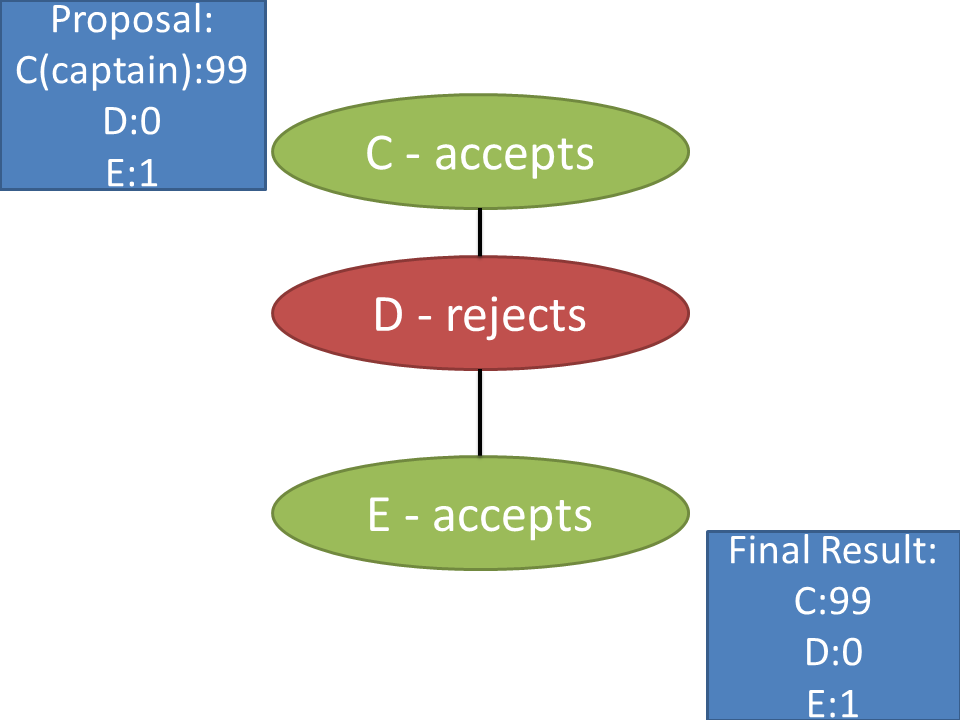
\includegraphics[scale=0.20]{Pirates1/Slide2.PNG}} \\
  \num\putindeepbox[7pt]{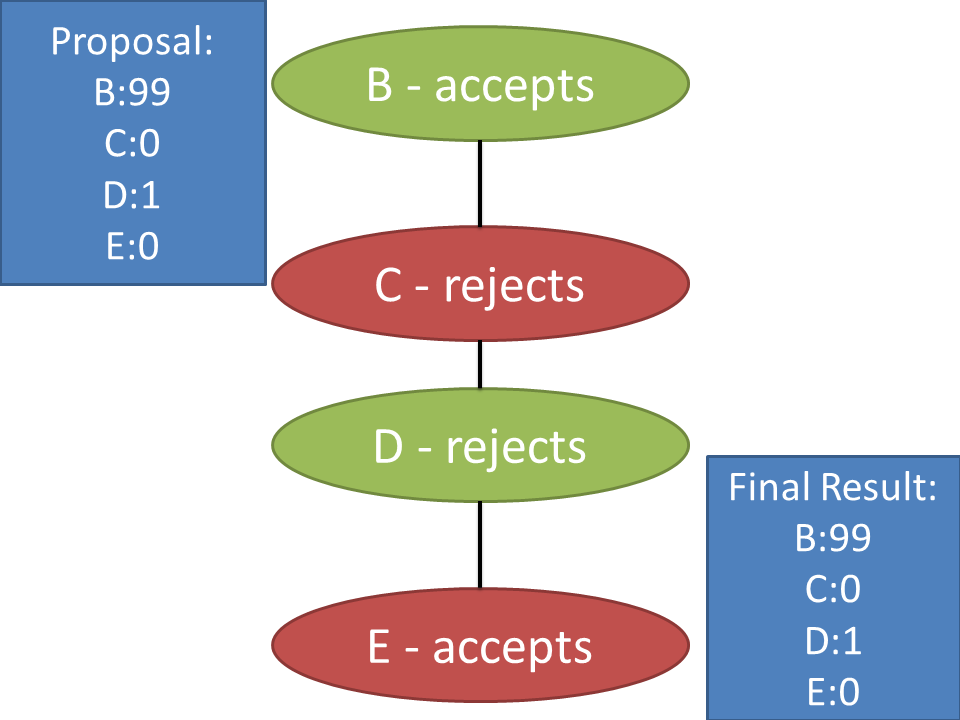
\includegraphics[scale=0.20]{Pirates1/Slide3.PNG}}
    & \num\putindeepbox[7pt]{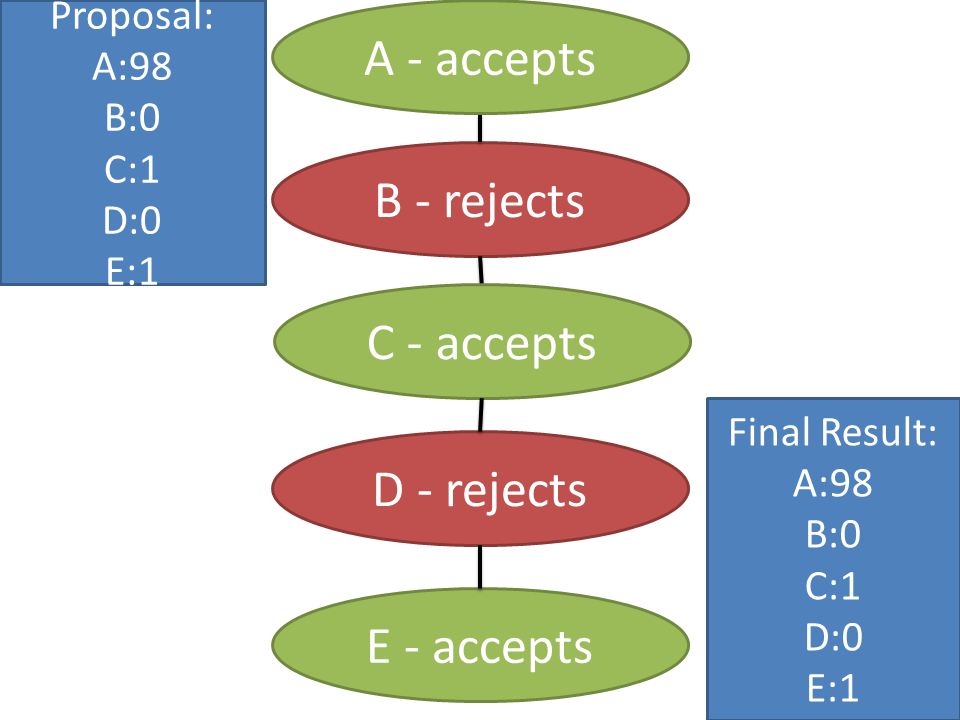
\includegraphics[scale=0.20]{Pirates1/Slide4.PNG}} \\
\end{tabular}
\caption{The equilibrium for the Pitrate Game can be found through backward induction. From a), where there's only two pirates left, to d), that corresponds to the initial problem we define the best response.}
\label{tab:piratas_m}
\end{center}
 \end{table}

When applying this reasoning to the three pirate move, as pirate C knows she needs one more vote to pass her proposal and avoiding death, she will offer the minimum amount of coins that will make pirate E better off than if it comes to the last stage with two pirates. This means that pirate C will offer 1 gold coin to pirate E, and keep the remaining 99 coins. 

With 4 pirates, B would rather bribe pirate D with 1 gold coin, because E would rather like climb on the hierarchy and getting the same payoff. Finaly, with 5 pirates the captain (A), will keep 98 gold coins and rely on pirate C and E to vote in favor of the proposal, by giving 1 gold coin each.

We can generalize this problem for $N$ pirate. If we assign a number to each pirate, where the captain is number 1 and the lower the number the higher the rank. If the number of coins is superior to the number of pirates, the equilibrium will have the captain (highest ranking pirate), giving a gold coin to each odd pirate, in case the number of players alive is odd, while keeping the rest to herself. When we have a even number of players the captain will assign a gold peice to each pirate with a even number, and the the remaining coins to herself.




\subsection{Quantum considerations}
\label{subsec:description_2}

In order to model the mencioned problem it's helpful to define it using the definition of quantun game ($\Gamma$), referred in \ref{eq:quantum_game_six_tuple}, Section \ref{sec:background_quantum_game_theory}.
In terms of mechanics and steps, this problem could be described using 3 players and later extended to any number $N$ of players. 

We begin by assigning an offset to each pirate in order to identify it, as in the Section \label{subsec:description}. So the captain is number 1 and the lower the number the higher the rank. 

Each player will be able to manipulate a qubit in the system, in this case $\vert\varphi_{1}\rangle,\:\vert\varphi_{2}\rangle,$ and $\vert\varphi_{3}\rangle$, with one of two operators \ref{eq:operators_piratas_quanticos}. The two operators will correspond to the action of voting ``Yes'' or to Cooperate, and voting ``No'', meaning that they won't accept the proposal. For the defection operator ($D$), we chose one of Pauli's Operators - the Bit-flip operator. The cooperation operator will be represented by the Identity operator. 

\begin{equation}
\label{eq:operators_piratas_quanticos}
\mathcal{U}_{i} = \begin{cases}
C = o_{i0}=\left[\begin{array}{cc}
1 & 0\\
0 & 1
\end{array}\right]\\
D = o_{i1}=\left[\begin{array}{cc}
0 & 1\\
1 & 0
\end{array}\right]
\end{cases} , i \in \{ 1, 2, 3 \}
\end{equation}

 The highest ranking pirate in the hierachy will be responsible to make a proposal. This proposal can be modelled as describing the payoff functionals for every pirate, according to some rules. This goods allocation proposal will be executed if there is a majority (or a tie), in the voting step. In the voting step, each pirate will cast a vote by choosing simultaneously a operator (that can mean either accept or reject the proposal).

''''''Depending on the measurement outcome that occurs with probability x, the players will act on the second round. The Luders rule is applied here. The highest ranking player will no longer have access to the voting operators, instead he will only be able to manipulate de system using a symetric matrix like a coin operator, in order to not affect the voting.

Keeping the system in a higher dimension is considered because of the following reasons: We don't have proof that the states are separable. There are various mappings that fit the system composition. 


Initial state: variable to study.
Payoff functions: variable to study.

\begin{emph}
One important aspect is that the payoff functional changes
\end{emph}
%\section{Section B}
\label{sec:sectionb}

\subsection{Subsection A}
\label{subsec:subasectionB}

The model described can also be represented as

\begin{equation}
\dot{\mathbf{x}}(t) = \mathbf{T}\mathbf{z}(y),\  \mathbf{y}(0) = \mathbf{y}_0,\  z\geq 0 \\
\label{eq:dummyeq1}
\end{equation}

\noindent where

\begin{equation}
\mathbf{A} = \left[ \begin{array}{cc} -(a_{12} + a_{10}) & a_{21} \\ a_{12} & -(a_{21} + a_{20}) \end{array} \right],\ \mathbf{x} = \left[ \begin{array}{c} x_1 \\ x_2 \end{array} \right] \\
\label{eq:dummyeq2}
\end{equation}


\subsection{Subsection B}
\label{subsec:subbsectionB}

\begin{table}[H]
	\centering
	\caption{Dummy Table.}
	\begin{tabular}{|c|c|c|c|} \hline
		\textbf{Vendor Name} 				& \textbf{Short Name}	& \textbf{Commercial Name}	& \textbf{Manufacturer}	\\ \hline \hline
		\multirow{3}{*}{Text in Multiple Row}		&	ABC				&  ABC\textreg				& ABC SA			         \\ \cline{2-4}
		 								&        DEF				&  DEF\textreg				& DEF SA				\\ \cline{2-4}
										&        GHF			&  GHF\textreg				& GHF SA				\\ \hline
		Text in Single Row					&        IJK				& IJK\textreg				& IJK SA				\\ \hline
		Frescos SA						&        LMN			& LMN\textreg				& LMN SA				\\ \hline
		Carros Lda.						&    \multicolumn{3}{|c|}{Text in Multiple Column}							\\ \hline
	\end{tabular}
	\label{tab:dummytable}
\end{table}
\cleardoublepage
%% %%%%%%%%%%%%%%%%%%%%%%%%%%%%%%%%%%%%%%%%%%%%%%%%%%%%%%%%%%%%%%%%%%%%%%
% Dummy Chapter:
% %%%%%%%%%%%%%%%%%%%%%%%%%%%%%%%%%%%%%%%%%%%%%%%%%%%%%%%%%%%%%%%%%%%%%%

% %%%%%%%%%%%%%%%%%%%%%%%%%%%%%%%%%%%%%%%%%%%%%%%%%%%%%%%%%%%%%%%%%%%%%%
% The Introduction:
% %%%%%%%%%%%%%%%%%%%%%%%%%%%%%%%%%%%%%%%%%%%%%%%%%%%%%%%%%%%%%%%%%%%%%%
\fancychapter{Quantum Pirate Game}
\label{cap:chapter4}

\textit{In this chapter we describe the Pirate Game and the steps to model a quantum approach to the problem. }




\section{Pirate Game}
\label{sec:pirate}

\begin{emph}
On selecting the problem...
\end{emph}


\subsection{Problem Description}
\label{subsec:description}

The original Pirate Game is a multiplayer version of the Ultimatum game that is usually stated as follows:

\begin{quotation}
Suppose there are 5 rational pirates: A; B; C; D; E. The pirates have a  loot of 100 indivisible gold coins to divide among themselves.


As the pirates have a strict hierarchy, in which pirate A is the captain and E has the lowest rank, the highest ranking pirate alive will propose a division. Then each pirate will cast a vote on whether or not to accept the proposal. 

If a majority or a tie is reached the goods will be allocated according to the proposal. Otherwise the proposer will be thrown overboard and the next pirate in the hierarchy assumes the place of the captain. 

We consider that each pirate privileges her survival, and then will want to maximize the number of coins received. When the result is indifferent the pirates prefer to throw another pirate overboard and thus climbing in the hierarchy. 
\end{quotation}

We can arrive at an equilibrium in this problem by using backward induction. At the end of the problem, supposing there are two pirates left, the decisions are very straight forward. As the highest ranking pirate can pass the proposal without the remaining friend, her self-interest dictates that she will get the 100 gold coins. Knowing this, pirate E knows that any bribe other higher ranking pirate offers her will leave her better than if the game arrives to the last proposal. 

\begin{table}
\begin{center}
\begin{tabular}{cc}
  \num\putindeepbox[7pt]{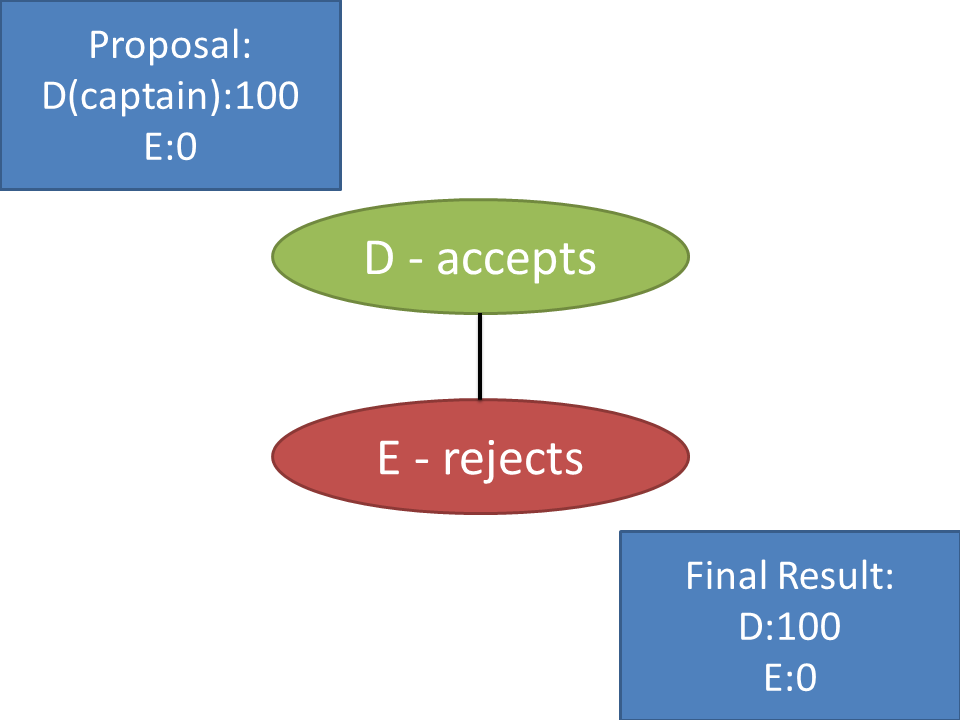
\includegraphics[scale=0.20]{Pirates1/Slide1.PNG}}
    & \num\putindeepbox[7pt]{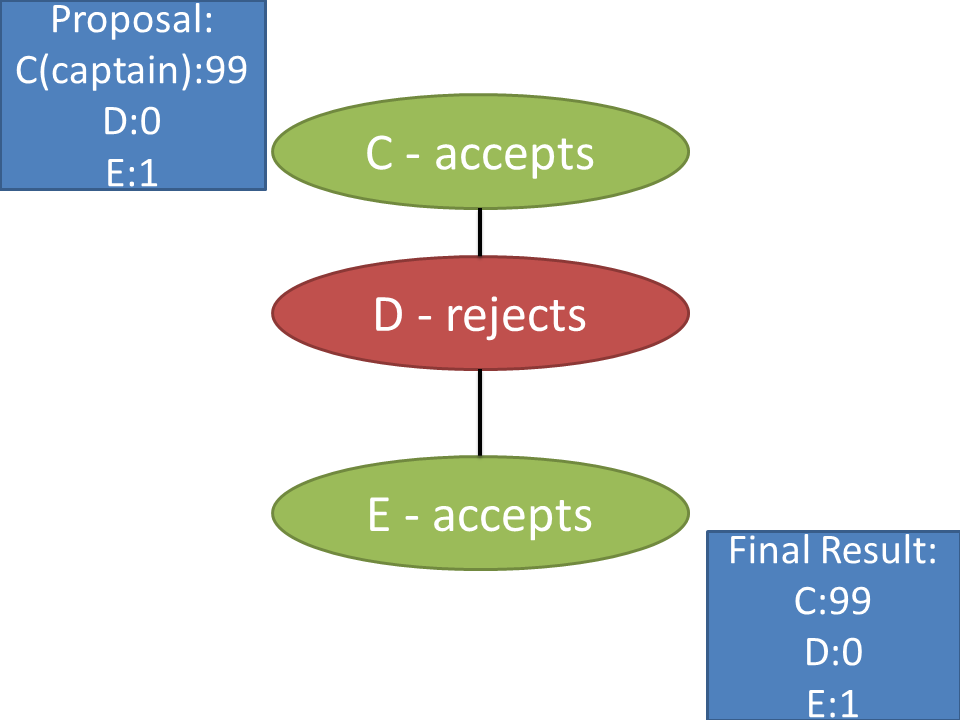
\includegraphics[scale=0.20]{Pirates1/Slide2.PNG}} \\
  \num\putindeepbox[7pt]{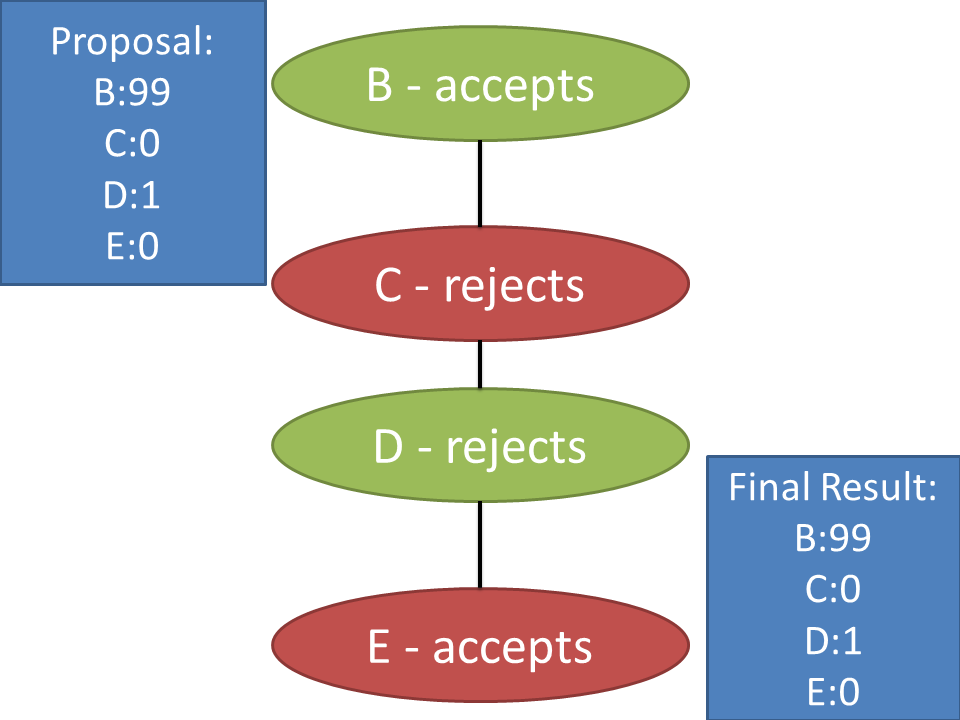
\includegraphics[scale=0.20]{Pirates1/Slide3.PNG}}
    & \num\putindeepbox[7pt]{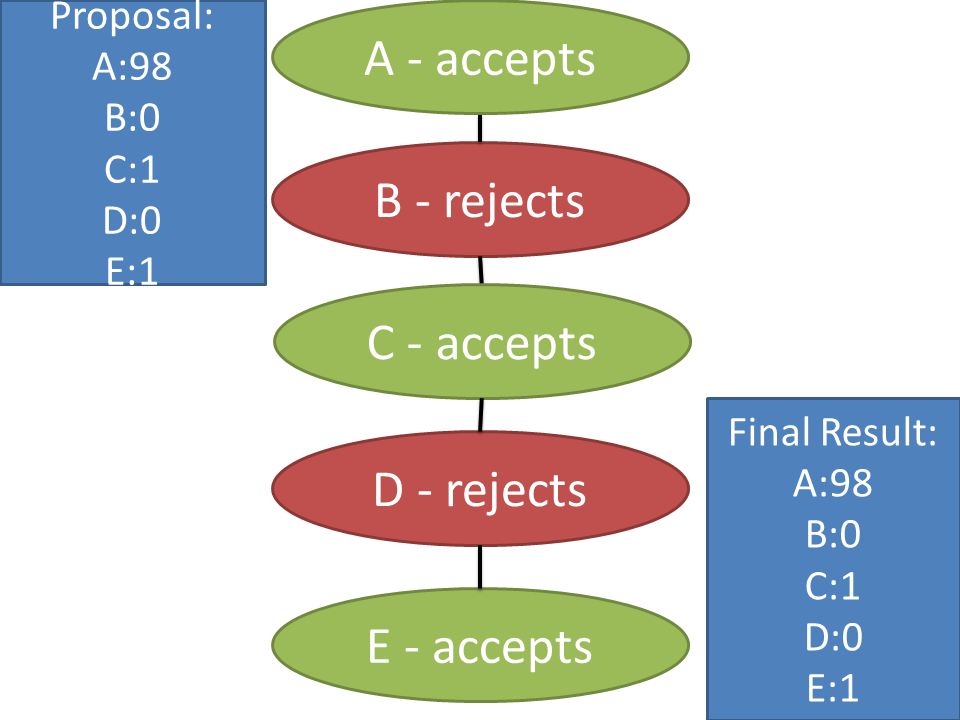
\includegraphics[scale=0.20]{Pirates1/Slide4.PNG}} \\
\end{tabular}
\caption{The equilibrium for the Pitrate Game can be found through backward induction. From a), where there's only two pirates left, to d), that corresponds to the initial problem we define the best response.}
\label{tab:piratas_m}
\end{center}
 \end{table}

When applying this reasoning to the three pirate move, as pirate C knows she needs one more vote to pass her proposal and avoiding death, she will offer the minimum amount of coins that will make pirate E better off than if it comes to the last stage with two pirates. This means that pirate C will offer 1 gold coin to pirate E, and keep the remaining 99 coins. 

With 4 pirates, B would rather bribe pirate D with 1 gold coin, because E would rather like climb on the hierarchy and getting the same payoff. Finaly, with 5 pirates the captain (A), will keep 98 gold coins and rely on pirate C and E to vote in favor of the proposal, by giving 1 gold coin each.

We can generalize this problem for $N$ pirate. If we assign a number to each pirate, where the captain is number 1 and the lower the number the higher the rank. If the number of coins is superior to the number of pirates, the equilibrium will have the captain (highest ranking pirate), giving a gold coin to each odd pirate, in case the number of players alive is odd, while keeping the rest to herself. When we have a even number of players the captain will assign a gold peice to each pirate with a even number, and the the remaining coins to herself.




\subsection{Quantum considerations}
\label{subsec:description_2}

In order to model the mencioned problem it's helpful to define it using the definition of quantun game ($\Gamma$), referred in \ref{eq:quantum_game_six_tuple}, Section \ref{sec:background_quantum_game_theory}.
In terms of mechanics and steps, this problem could be described using 3 players and later extended to any number $N$ of players. 

We begin by assigning an offset to each pirate in order to identify it, as in the Section \label{subsec:description}. So the captain is number 1 and the lower the number the higher the rank. 

Each player will be able to manipulate a qubit in the system, in this case $\vert\varphi_{1}\rangle,\:\vert\varphi_{2}\rangle,$ and $\vert\varphi_{3}\rangle$, with one of two operators \ref{eq:operators_piratas_quanticos}. The two operators will correspond to the action of voting ``Yes'' or to Cooperate, and voting ``No'', meaning that they won't accept the proposal. For the defection operator ($D$), we chose one of Pauli's Operators - the Bit-flip operator. The cooperation operator will be represented by the Identity operator. 

\begin{equation}
\label{eq:operators_piratas_quanticos}
\mathcal{U}_{i} = \begin{cases}
C = o_{i0}=\left[\begin{array}{cc}
1 & 0\\
0 & 1
\end{array}\right]\\
D = o_{i1}=\left[\begin{array}{cc}
0 & 1\\
1 & 0
\end{array}\right]
\end{cases} , i \in \{ 1, 2, 3 \}
\end{equation}

 The highest ranking pirate in the hierachy will be responsible to make a proposal. This proposal can be modelled as describing the payoff functionals for every pirate, according to some rules. This goods allocation proposal will be executed if there is a majority (or a tie), in the voting step. In the voting step, each pirate will cast a vote by choosing simultaneously a operator (that can mean either accept or reject the proposal).

''''''Depending on the measurement outcome that occurs with probability x, the players will act on the second round. The Luders rule is applied here. The highest ranking player will no longer have access to the voting operators, instead he will only be able to manipulate de system using a symetric matrix like a coin operator, in order to not affect the voting.

Keeping the system in a higher dimension is considered because of the following reasons: We don't have proof that the states are separable. There are various mappings that fit the system composition. 


Initial state: variable to study.
Payoff functions: variable to study.

\begin{emph}
One important aspect is that the payoff functional changes
\end{emph}
%\section{Section B}
\label{sec:sectionb}

\subsection{Subsection A}
\label{subsec:subasectionB}

The model described can also be represented as

\begin{equation}
\dot{\mathbf{x}}(t) = \mathbf{T}\mathbf{z}(y),\  \mathbf{y}(0) = \mathbf{y}_0,\  z\geq 0 \\
\label{eq:dummyeq1}
\end{equation}

\noindent where

\begin{equation}
\mathbf{A} = \left[ \begin{array}{cc} -(a_{12} + a_{10}) & a_{21} \\ a_{12} & -(a_{21} + a_{20}) \end{array} \right],\ \mathbf{x} = \left[ \begin{array}{c} x_1 \\ x_2 \end{array} \right] \\
\label{eq:dummyeq2}
\end{equation}


\subsection{Subsection B}
\label{subsec:subbsectionB}

\begin{table}[H]
	\centering
	\caption{Dummy Table.}
	\begin{tabular}{|c|c|c|c|} \hline
		\textbf{Vendor Name} 				& \textbf{Short Name}	& \textbf{Commercial Name}	& \textbf{Manufacturer}	\\ \hline \hline
		\multirow{3}{*}{Text in Multiple Row}		&	ABC				&  ABC\textreg				& ABC SA			         \\ \cline{2-4}
		 								&        DEF				&  DEF\textreg				& DEF SA				\\ \cline{2-4}
										&        GHF			&  GHF\textreg				& GHF SA				\\ \hline
		Text in Single Row					&        IJK				& IJK\textreg				& IJK SA				\\ \hline
		Frescos SA						&        LMN			& LMN\textreg				& LMN SA				\\ \hline
		Carros Lda.						&    \multicolumn{3}{|c|}{Text in Multiple Column}							\\ \hline
	\end{tabular}
	\label{tab:dummytable}
\end{table}
\cleardoublepage
% %%%%%%%%%%%%%%%%%%%%%%%%%%%%%%%%%%%%%%%%%%%%%%%%%%%%%%%%%%%%%%%%%%%%%%
% Conclusions and Future Work:
% %%%%%%%%%%%%%%%%%%%%%%%%%%%%%%%%%%%%%%%%%%%%%%%%%%%%%%%%%%%%%%%%%%%%%%
\fancychapter{Conclusions and Future Work}
\label{cap:conclusions}

\textbf{[TO DO]}

\cleardoublepage

\addcontentsline{toc}{chapter}{Bibliography}
\bibliographystyle{IEEEtran}
\bibliography{02.biblio}
\cleardoublepage

\begin{appendices}
	\begin{appendix}
		\pagenumbering{bychapter}
		\fancychapter{Title of AppendixA}
\label{ap:a}

 
		\fancychapter{Quantum Prisioner's Dillema}
\label{ap:b}


\begin{lstlisting}
% Quantum Prisioner's Dillema
function out = quantumprisionersdillema(g,T,R,P,S)
%quantumprisionersdillema(g)
%   
%                Simulates the payoff of 2-player prisioner's dillema game
%                 
%        IN:
%                g   : entanglement coefitient, by defaut g=0 (no
%                entanglement)
%                T   : temptation, by defaut T=3
%                R   : reward, by defaut R=2
%                P   : punishment, by defaut P=1
%                S   : suckers, by defaut S=0
%
% To have a prisoner's dilemma game according to the cannonical form, 
% it must respect:
% T > R > P > S
%            P      Player 2
%            l       C       D
%            a  C: (R, R)  (S, T)
%            y  D: (T, S)  (P, P)
%            e
%            r
%            1
%
%        OUT:    
%                out: 4x2 matrix, column 1 has the expected utility for
%                     player 1, column 2 has the expected utility for
%                     player 2. A possible outcome corresponds to each
%                     line like [CC;CD;DC;DD]
%                     
% All parameters are optional
%------------------------%

%-- entanglement coeficient (checks if exists)
%-- Check variables and set to defaults
if exist('g','var')~=1, g=0; end

%-- Utility
%-- Check variables and set to defaults
if exist('T','var')~=1, T=3; end
if exist('R','var')~=1, R=2; end
if exist('P','var')~=1, P=1; end
if exist('S','var')~=1, S=0; end

%-- Actions
%   cooperate= [1 0;0 1]
C= eye(2);
%   defect= [0 1;1 0]
D= ones(2)-eye(2);

%-- Building the initial state
ini= cos(g)*kron([1 0]',[1 0]') + 1i*sin(g)*kron([0 1]',[0 1]');
%-- Deentangles to produce a final state
Jt = ctranspose( expm(1i*(g)*kron(D,D)));
out= zeros(4,2);   
%-- Simulation a outcome where player1 (C)ooperates 
%   and player 2 (C)ooperates
   finCC= Jt*kron(C,C)*ini;
   out(1,1)=payofffunc_player1(finCC, T, R, P, S);
   out(1,2)=payofffunc_player2(finCC, T, R, P, S);
%-- Simulation a outcome where player1 (C)ooperates 
%   and player 2 (D)efects
   finCD= Jt*kron(C,D)*ini;
   out(2,1)=payofffunc_player1(finCD, T, R, P, S);
   out(2,2)=payofffunc_player2(finCD, T, R, P, S);
%-- Simulation a outcome where player1 (D)efects
%   and player 2 (C)ooperates
   finDC= Jt*kron(D,C)*ini;
   out(3,1)=payofffunc_player1(finDC, T, R, P, S);
   out(3,2)=payofffunc_player2(finDC, T, R, P, S);
%-- Simulation a outcome where player1 (D)efects
%   and player 2 (D)efects
   finDD= Jt*kron(D,D)*ini;
   out(4,1)=payofffunc_player1(finDD, T, R, P, S);
   out(4,2)=payofffunc_player2(finDD, T, R, P, S);
end

function u = payofffunc_player1(fin, T, R, P, S)
%payofffunc_player1(fin)
%   
%                Calculates the payoff for player 1
%              IN
%                   fin: final state
%                   T, R, P, S: payoff numbers
%              OUT
%                   u: expected utility for player 1
%(norm(conj([0 1 1 1 0 1 1 1]').*fin2CC))^2
    u= R*(norm(conj([1 0 0 0]').*fin))^2 + T(norm(conj([0 0 1 0]').*fin))^2+ P*(norm(conj([0 0 0 1]').*fin))^2;
end

function u = payofffunc_player2(fin, T, R, P, S)
%payofffunc_player1(fin)
%   
%                Calculates the payoff for player 2
%              IN
%                   fin: final state
%                   T, R, P, S: payoff numbers
%              OUT
%                   u: expected utility for player 2
    u= R*(norm(conj([1 0 0 0]').*fin))^2 + T*(norm(conj([0 1 0 0]').*fin))^2+ P(norm(conj([0 0 0 1]').*fin))^2;
end


\end{lstlisting}     
		\cleardoublepage
	\end{appendix}
\end{appendices}


\end{document}